% Memoria TNyCA 2026-27: ruta LEMD 36R -> LLBG 21, B738
% Compilar: latexmk -pdf main.tex   (tablas: python3 gen_tablas.py, previo xlsx2csv.m)
\documentclass[11pt,a4paper]{article}
\usepackage[utf8]{inputenc}
\usepackage[T1]{fontenc}
\usepackage{lmodern}
\usepackage[spanish,es-tabla,es-noshorthands]{babel}
\usepackage[margin=2cm,top=2.3cm,bottom=2.3cm]{geometry}
\usepackage{graphicx,booktabs,longtable,tabularx,array,xcolor,amsmath,amssymb}
\usepackage{caption,float,enumitem,microtype,fancyhdr,makecell,needspace}
\usepackage[hidelinks]{hyperref}
\graphicspath{{fig/}}
\newcommand{\enrFijos}{26}
\newcommand{\enrDist}{1\,852,1}
\newcommand{\enrTnoW}{4:06:57}
\newcommand{\enrTnoWh}{4,12}
\newcommand{\enrDistW}{1\,744,3}
\newcommand{\enrTW}{3:52:35}
\newcommand{\enrTWh}{3,88}
\newcommand{\enrTWg}{3:38:39}
\newcommand{\enrTWgh}{3,64}
\newcommand{\enrGSmin}{458}
\newcommand{\enrGSmax}{496}
\newcommand{\enrGSmed}{479}
\newcommand{\enrDevMax}{23,4}
\newcommand{\enrDevMaxFix}{ADEXI}
\newcommand{\enrDevZukko}{0,79}
\newcommand{\enrDiffW}{14}
\newcommand{\enrDiffWg}{28}
\newcommand{\enrDeltaD}{107,8}
\newcommand{\enrWcaMax}{4,3}
\newcommand{\loxDA}{377}
\newcommand{\loxA}{14,7}
\newcommand{\loxLegA}{OLLEK--NEVIK}
\newcommand{\loxDB}{291}
\newcommand{\loxB}{8,8}
\newcommand{\loxLegB}{IBREP--ADEXI}
\newcommand{\loxRestD}{216}
\newcommand{\loxRest}{4,0}
\newcommand{\misCAtrk}{208,7}
\newcommand{\misCAdist}{2,99}
\newcommand{\misTurn}{3,40}
\newcommand{\misDF}{7,60}
\newcommand{\sidDist}{92,7}
\newcommand{\sidN}{8}
\newcommand{\sidCA}{1,50}
\newcommand{\sidMDVIIIIIIValt}{15\,660}
\newcommand{\sidMDOIVVIIalt}{3\,291}
\newcommand{\sidMDOIVVIIIalt}{7\,501}
\newcommand{\sidMDOIVIXalt}{9\,165}
\newcommand{\sidMDVIIIIIIVD}{40,9}
\newcommand{\arrDist}{92,5}
\newcommand{\arrTotal}{108,5}
\newcommand{\arrToppuRest}{16,0}
\newcommand{\misDist}{14,0}
\newcommand{\ilsN}{4}
\newcommand{\rnpN}{11}
\newcommand{\rnpDist}{38,7}
\newcommand{\rnpArc}{1,26}
\newcommand{\rnpGintuLeg}{11,9}
\newcommand{\ilsGalgaLeg}{6,5}
\newcommand{\ilsFapLeg}{2,06}
\newcommand{\ilsFinal}{7,45}
\newcommand{\rnpFinal}{3,15}
\newcommand{\ilsGPdeg}{3,06}
\newcommand{\vTOC}{145,1}
\newcommand{\vTOD}{1\,881,8}
\newcommand{\vNlegs}{22}
\newcommand{\vNclb}{9}
\newcommand{\vNcru}{3}
\newcommand{\vNdes}{10}
\newcommand{\vFuelClb}{1\,985}
\newcommand{\vFuelCru}{9\,711}
\newcommand{\vFuelDes}{747}
\newcommand{\vFuelTot}{12\,443}
\newcommand{\vTime}{4:58:23}
\newcommand{\vTimeh}{4,97}
\newcommand{\vTclb}{23,7}
\newcommand{\vTdes}{34,2}
\newcommand{\vMldg}{63\,978}
\newcommand{\vMtoc}{74\,436}
\newcommand{\vMtod}{64\,725}
\newcommand{\vMcruMed}{69\,580}
\newcommand{\vHcru}{34\,982}
\newcommand{\vMcru}{0,752}
\newcommand{\vIAScru}{254}
\newcommand{\vTAScru}{433}
\newcommand{\vHcrossClb}{29\,315}
\newcommand{\vHcrossDes}{30\,889}
\newcommand{\vVIIpIIO}{172}
\newcommand{\vVref}{138}
\newcommand{\vVfap}{143}
\newcommand{\vTrKIIini}{81,2}
\newcommand{\vTrKIIfin}{74,3}
\newcommand{\vTrCII}{99,5}
\newcommand{\vTrCIVmax}{100,0}
\newcommand{\vTrIdle}{8,74}
\newcommand{\vTrDIII}{12,7}
\newcommand{\vTrDIIIV}{5,1}
\newcommand{\vTrDIIi}{27,7}
\newcommand{\vFPADIIi}{$-$0,81}
\newcommand{\vVSCI}{1\,815}
\newcommand{\vVSDIVI}{$-$3\,271}
\newcommand{\vVSDIVII}{$-$2\,214}
\newcommand{\vFPADI}{$-$3,06}
\newcommand{\vFPADIII}{$-$1,62}
\newcommand{\vFPADIIIII}{$-$2,06}
\newcommand{\vMDVIIIIIIVh}{20\,789}
\newcommand{\vMDOIVVIIIh}{11\,067}
\newcommand{\vCruiseLen}{1\,728,8}
\newcommand{\vDIVIlen}{9,4}
\newcommand{\vDIVIIlen}{53,6}
\newcommand{\vKIlen}{1,8}
\newcommand{\vKIIIlen}{6,0}
\newcommand{\vCItop}{3\,498}
\newcommand{\vCIItop}{4\,998}
\newcommand{\vCIIIVh}{21\,983}
\newcommand{\vTotalD}{2\,053,3}
\newcommand{\vDesLen}{171,6}
\newcommand{\cHI}{34\,982}
\newcommand{\cHII}{31\,000}
\newcommand{\cMRCI}{12\,443}
\newcommand{\cLRCI}{12\,543}
\newcommand{\cMRCII}{12\,942}
\newcommand{\cLRCII}{13\,051}
\newcommand{\cMachLRCI}{0,810}
\newcommand{\cMachMRCII}{0,687}
\newcommand{\cMachLRCII}{0,742}
\newcommand{\cTMRCI}{4,97}
\newcommand{\cTLRCI}{4,68}
\newcommand{\cTMRCII}{5,28}
\newcommand{\cTLRCII}{4,96}
\newcommand{\cDiffLRCI}{99}
\newcommand{\cDiffH}{498}
\newcommand{\cDiffTLRCI}{17}
\newcommand{\cTOCII}{110,1}
\newcommand{\chkN}{44}
\newcommand{\chkOK}{44}
\newcommand{\chkZukkoH}{13\,000}
\newcommand{\chkZukkoIAS}{290}
\newcommand{\chkMDVIIIIIIV}{20\,789}
\newcommand{\chkMDVIIIIIIVmin}{15\,660}
\newcommand{\chkNANDO}{28\,612}
\newcommand{\chkPIKOG}{20\,720}
\newcommand{\vTODzukko}{63,0}
\newcommand{\sbBurn}{12\,180}
\newcommand{\sbTOW}{76\,421}
\newcommand{\sbLDW}{64\,241}
\newcommand{\sbTime}{4:24:16}
\newcommand{\sbTimeh}{4,40}
\newcommand{\sbAirac}{2503}
\newcommand{\sbDist}{2\,031}
\newcommand{\sbCI}{80}
\newcommand{\sbSteps}{LEMD/\allowbreak 0320/\allowbreak IBREP/\allowbreak 0330/\allowbreak NEVIK/\allowbreak 0350}
\newcommand{\sbDiffFuel}{263}
\newcommand{\sbDiffFuelPct}{2,2}
\newcommand{\sbDiffLDW}{$-$263}
\newcommand{\sbMZFW}{62\,732}
\newcommand{\sbMTOW}{78\,541}
\newcommand{\sbPax}{180}
\newcommand{\sbMach}{.80}
\newcommand{\sbTAS}{465}
\newcommand{\sbRoute}{NAND6W NANDO DCT FENXE T257 LASPO DCT ORVUS DCT GODOX DCT EDULI DCT PTC DCT SOTAX DCT RISEP DCT ETOIL DCT XATOS DCT IBREP DCT ADEXI DCT OLLEK DCT NEVIK UL144 PLH UM978 SIT DCT VANZA DCT PIKOG L609 ZUKKO AMOS1B}

\captionsetup{font=small,labelfont=bf,width=0.95\linewidth,justification=raggedright}
\setlength{\parskip}{3pt plus 1pt}
\setlength{\emergencystretch}{2.5em}
\setlength{\LTcapwidth}{0.95\linewidth}
% Flotantes: admitir figuras/tablas grandes junto al texto, sin páginas medio vacías
\renewcommand{\topfraction}{0.9}\renewcommand{\bottomfraction}{0.8}
\renewcommand{\textfraction}{0.07}\renewcommand{\floatpagefraction}{0.8}
\setlist{nosep}
\pagestyle{fancy}\fancyhf{}
\fancyhead[L]{\small TNyCA -- Ruta LEMD 36R $\rightarrow$ LLBG 21 (B738)}\fancyhead[R]{\small Eden Rochman Sharabi}
\fancyfoot[C]{\thepage}
\renewcommand{\headrulewidth}{0.3pt}

% Cuadro para lo que el estudiante debe comprobar contra el AIP correspondiente
\newcommand{\pendiente}[1]{\par\medskip\noindent\fcolorbox{red}{red!4}{\parbox{\dimexpr\linewidth-2\fboxsep-2\fboxrule}{%
\textcolor{red}{\textbf{PENDIENTE DE VERIFICAR.}} #1}}\par\medskip}
\newcommand{\ok}{\textcolor{green!50!black}{\textbf{VERIFICADO}}}
\newcommand{\nok}{\textcolor{red}{\textbf{PENDIENTE}}}
% Columnas p/X en bandera (sin huecos de justificación)
\newcolumntype{L}[1]{>{\raggedright\arraybackslash}p{#1}}
\newcolumntype{Y}{>{\raggedright\arraybackslash}X}
% Formato del apendice B del enunciado; longtable: corta entre filas
\newcommand{\funcion}[4]{\par\Needspace{8\baselineskip}\begingroup\setlength{\LTleft}{0pt}\setlength{\LTright}{0pt}%
\setlength{\LTpre}{2mm}\setlength{\LTpost}{3mm}%
\begin{longtable}{@{}>{\bfseries\raggedright\arraybackslash}p{3.3cm}L{\dimexpr\linewidth-3.3cm-2\tabcolsep\relax}@{}}\toprule
Función: & \texttt{#1}\\* \midrule
Parámetros de entrada: & #2\\ \midrule
Parámetros de salida: & #3\\ \midrule
Funcionamiento: & #4\\ \bottomrule
\end{longtable}\addtocounter{table}{-1}\endgroup}
% Nombres de código: se permite cortar la línea tras «_»
\DeclareRobustCommand{\m}[1]{{\ttfamily\def\_{\textunderscore\penalty100\relax}#1}}

\begin{document}

% ============================================================ PORTADA
\begin{titlepage}
\centering
{\large Universitat Politècnica de València\\ Escuela Técnica Superior de Ingeniería del Diseño\\[2mm] Grado en Ingeniería Aeroespacial\par}
\vspace{1.2cm}
{\Large Transporte, Navegación y Circulación Aérea\par}
\vspace{2.5cm}
{\LARGE\bfseries Cálculo de una ruta aérea\par}
\vspace{4mm}
{\Large Madrid-Barajas (LEMD, pista 36R) $\rightarrow$ Tel Aviv-Ben Gurión (LLBG, pista 21)\par}
\vspace{3mm}
{\large Boeing 737-800 (B738), modelo BADA 3.14\par}
\vspace{2.5cm}
{\large\bfseries Eden Rochman Sharabi\par}
\vspace{1cm}
{\large Curso 2026--2027\\ Entrega: 22 de diciembre de 2026\par}
\vfill
{\small Memoria del trabajo de la asignatura. Software MATLAB R2026b, bibliotecas \texttt{kgbx-lib} (geo, kml, bada) y BADA 3.14 proporcionadas en el curso.\par}
\end{titlepage}

\tableofcontents
\clearpage

% ============================================================ 1
\section{Introducción y objetivos}

El objetivo del trabajo es calcular una ruta aérea completa entre dos aeródromos a partir de la documentación oficial (AIP), dividiéndola en las fases de salida (SID), en-ruta, llegada (STAR/transición) y aproximación, y proponer para ella un perfil vertical coherente con las prestaciones del avión y con las restricciones de las cartas. Siguiendo el enunciado, la memoria se organiza en capítulos por fase de vuelo, empezando por la fase de crucero, y para cada fase se dan:

\begin{enumerate}
\item la lista de fijos y tramos con sus coordenadas y distancias, obtenidos de las cartas y comprobados contra ellas (secciones~\ref{sec:crucero} a~\ref{sec:llegada});
\item las restricciones de altitud y velocidad de cada fijo y su representación gráfica (perfil vertical mínimo/máximo);
\item los ficheros KML (Google Earth) y las tablas Excel generadas con MATLAB.
\end{enumerate}

Además se calcula el tiempo de la fase en-ruta sin viento y con el viento previsto en el plan de vuelo LIDO (SimBrief) resolviendo el triángulo de velocidades con la función \m{computeWT} (sección~\ref{sec:viento}); se propone un perfil vertical ascenso--crucero--descenso con tramos SPD y PTH usando el modelo de energía total de BADA~3.14 para el B738 (sección~\ref{sec:vertical}); y se comparan los consumos para dos altitudes y dos velocidades de crucero.

Los entregables son: esta memoria, las cartas PDF con la ruta marcada, los ficheros KML y Excel de \m{matlab/out/}, y el código MATLAB (\m{matlab/main\_*.m} y \m{matlab/lib/}), explicado función por función en el apéndice~\ref{ap:funciones} con el formato del apéndice~B del enunciado. El apéndice~\ref{ap:otra-ruta} enumera los cambios necesarios para otra ruta, el apéndice~\ref{ap:supuestos} las suposiciones adoptadas y el apéndice~\ref{ap:verif} el estado de verificación de cada dato frente a las fuentes oficiales. Los datos que no han podido comprobarse contra un AIP se señalan en el texto con cuadros \textcolor{red}{\textbf{PENDIENTE DE VERIFICAR}}; no deben darse por buenos hasta completar esa comprobación.

\paragraph{Convención de las tablas.} Como en la figura~2 del enunciado y en su apéndice~B, cada fijo lleva los datos del tramo que \emph{llega} a él: \m{track} es la derrota desde el fijo anterior y \m{dist} la distancia desde el fijo anterior (el texto de la sección~3.1 del enunciado dice «distancia al siguiente fijo», pero la figura~2 muestra la otra convención: PINAR 0, SEGRE 10,41). En salida y en-ruta la columna «Distancia total» es la acumulada desde el origen; en llegada y aproximación es la distancia restante hasta el umbral, como pide la sección~5 del enunciado. Las distancias y derrotas son ortodrómicas (\m{orto\_distazi}, \m{orto\_reckon} de \m{kgbx-lib/geo}); los tiempos se expresan en segundos en las tablas Excel, como en la figura~2.

% ============================================================ 2
\section{Cálculo inicial de la ruta}

\subsection{Elección de la ruta y del avión}

\begin{table}[H]\centering\small
\begin{tabular}{llll}\toprule
 & Aeropuerto & Pista & Comentario\\ \midrule
ORG & LEMD & 36R & Madrid -- Adolfo Suárez Madrid-Barajas, pista 36 derecha\\
DST & LLBG & 21 & Tel Aviv -- Ben Gurión, pista 21\\ \bottomrule
\end{tabular}
\caption{Aeródromos y pistas de la ruta.}
\end{table}

\textbf{Ruta.} LEMD--LLBG es una ruta internacional de medio radio (\sbDist~NM según el plan SimBrief; \vTotalD~NM del DER 36R al umbral de la 21 según el cálculo de esta memoria) con demanda regular de pasajeros entre España e Israel, lo que justifica un avión de pasillo único de medio alcance. Atraviesa cinco FIR con espacio aéreo de ruta libre (España, Francia, Italia, Grecia y Chipre), lo que obliga a trabajar con la documentación de ruta libre además de las aerovías convencionales, y los dos aeródromos disponen de procedimientos RNAV de cierta complejidad: en LEMD se ha elegido la SID NANDO3R (en lugar de la PINAR4R del ejemplo del curso) y en LLBG la transición ERREZ1A, que tiene carta propia de transiciones a la aproximación, la aproximación de precisión ILS RWY 21 y la de no precisión RNP~Y RWY~21, que tiene un recorrido lateral distinto de la ILS (fijos VATAT/NAMIM y un tramo RF). Se descartó usar la LOC~21 como aproximación de no precisión porque comparte el recorrido lateral de la ILS~21.

\textbf{Avión.} Se ha elegido el Boeing 737-800 (OACI B738):
\begin{itemize}
\item \emph{Autonomía.} Con la masa de despegue estimada por SimBrief (\sbTOW~kg, \sbPax~pasajeros) el consumo calculado en la sección~\ref{sec:vertical} es \vFuelTot~kg para \vTotalD~NM, frente a una capacidad máxima de combustible de 20\,911~kg según el plan SimBrief (\m{max\_tanks}); el plan SimBrief estima 12\,180~kg de combustible de etapa. La ruta queda, por tanto, cómodamente dentro del alcance del avión.
\item \emph{Aeródromos.} Según AD~2~LEMD (AIP ENAIRE), la pista 36R mide 3\,500~m~$\times$~60~m, PCN 134/F/A/W/T, con elevación del umbral 1\,942~ft y del aeródromo 1\,998~ft. Según AD~2~LLBG (eAIP Israel), la pista 21 mide 2\,772~m~$\times$~60~m (TORA 2\,772~m, LDA 2\,772~m) y la elevación del aeródromo es 134~ft. BADA~3.14 da para el B738 una longitud de despegue de 2\,308~m y de aterrizaje de 1\,646~m (fichero \m{B738\_\_.OPF}, bloque \emph{ground}), por lo que ambas pistas son suficientes. Ninguno de los dos aeródromos restringe el tipo de avión más allá de la lista de tipos ruidosos de LEMD AD~2.21 (en la que no está el B738).
\item \emph{Datos disponibles.} El B738 está en BADA~3.14 (ficheros OPF, APF, PTF), es el avión del ejemplo del curso y del simulador, y existe abundante documentación operativa; SimBrief genera el plan LIDO para este tipo.
\end{itemize}

\subsection{Cartas de navegación utilizadas}

Todas las cartas proceden de los AIP oficiales y se entregan en PDF, con la ruta marcada, en la carpeta \m{cartas/}. La tabla~\ref{tab:cartas} indica la fuente, la fecha o ciclo AIRAC impreso en cada carta y si los datos usados en el cálculo se han comprobado contra ella. Dos advertencias:
\begin{itemize}
\item El plan de vuelo SimBrief (\m{simbrief/LEMDLLBG\_XML\_1793965869.xml}) se generó con la base de datos de navegación \textbf{AIRAC \sbAirac{} (marzo de 2025), obsoleta} respecto de las cartas. Su SID (NANDO6W) y su STAR (AMOS1B) no coinciden con los procedimientos vigentes (NANDO3R, ERREZ1A), por lo que del plan solo se han tomado los fijos del tramo en-ruta NANDO--ZUKKO y la previsión de viento. Todos los fijos de SID, transición y aproximaciones se han tomado de las cartas.
\item Las cartas de LEMD corresponden al AIP ENAIRE en vigor en el momento de la consulta (AD~2~LEMD con AIRAC AMDT 10/26, WEF 29-OCT-26) y las de LLBG al eAIP de Israel con AIRAC AMDT 001/2026 (06 AUG 2026). El ciclo AIRAC 002/2026 entra en vigor el 26 de noviembre de 2026, antes de la entrega: las cartas deberán recomprobarse en esa fecha.
\end{itemize}

\begin{table}[!htbp]\centering\footnotesize
\begin{tabularx}{\linewidth}{lL{4.0cm}L{2.6cm}YL{2.5cm}}\toprule
Fase & Carta & Fuente oficial & Fecha / AIRAC en la carta & Comprobado\\ \midrule
Salida & AD 2-LEMD SID 7 (RWY 36R: NANDO3R) & AIP ENAIRE, AD 2 LEMD & 30-OCT-25 (AMDT 399/25); pág. 7.3 WEF 20-MAR-25 AIRAC AMDT 02/25; pág. 7.5 WEF 12-JUN-25 AIRAC AMDT 05/25 & \ok\\
Salida & AD 2-LEMD, texto AD 2.21 y datos de pista & AIP ENAIRE & AIRAC AMDT 10/26, WEF 29-OCT-26 & \ok\\
En-ruta & ENR 3.2 (T257) y ENR 4.4 (fijos) & AIP ENAIRE & consulta nov-2026 & \ok{} NANDO--SOTAX\\
En-ruta & ENR 4.4 y FRA LFFRASE & AIP France (eAIP A-2026-10, 01 OCT 2026) & AIRAC 10/26 & \ok{} SOTAX, RISEP, ETOIL, XATOS\\
En-ruta & ENR 3 / ruta libre & AIP Italia (ENAV), Grecia, Chipre & -- & \nok{} (sección~\ref{sec:enr-pendiente})\\
Llegada & AD 2 LLBG TRANS 21-26 (ERREZ1A) & eAIP Israel & 18 MAY 23 & \ok\\
Llegada & AD 2 LLBG STAR 21-26 (esperas en ZUKKO) & eAIP Israel & 31 OCT 24 & \ok{} (consultada, no volada)\\
Aproximación & AD 2 LLBG IAC-21ILS-4 (ILS RWY 21) & eAIP Israel & 31 OCT 24, AIRAC AMDT 001/2024, CAA AMDT 3/24 & \ok\\
Aproximación & AD 2 LLBG IAC 21RNPY-3 (RNP Y RWY 21) & eAIP Israel & 06 AUG 2026, AIRAC AMDT 001/2026 & \ok\\
Aproximación & AD 2 LLBG (datos de pista, AD 2.21) & eAIP Israel & 06 AUG 2026, AIRAC AMDT 001/2026 & \ok\\ \bottomrule
\end{tabularx}
\caption{Cartas y documentos oficiales utilizados. «Comprobado» indica que las coordenadas, derrotas, distancias y restricciones usadas en el código se han cotejado con el documento.}
\label{tab:cartas}
\end{table}

\subsection{Perfil horizontal: lista de fijos por fase}

La tabla~\ref{tab:fijos} enumera los fijos de cada fase en el orden en que se vuelan, con el procedimiento o la ruta ATS a la que pertenecen.

\begin{table}[!htbp]\centering\footnotesize
\begin{tabularx}{\linewidth}{lL{3.6cm}Y}\toprule
Fase & Procedimiento / ruta & Fijos\\ \midrule
SID & NANDO3R (RWY 36R) & DER36R, CA2500 (fin del tramo CA a 2\,500 ft, calculado), MD047, MD048, MD049, MD824, MD922, NANDO\\
En-ruta & DCT & NANDO, FENXE\\
 & T257 & FENXE, MABUX, RETBA, MOPIR, LASPO\\
 & DCT (ruta libre España / Francia, FRA LFFRASE) & LASPO, ORVUS, GODOX, EDULI, PTC, SOTAX, RISEP, ETOIL, XATOS, IBREP\\
 & DCT (ruta libre Italia) & IBREP, ADEXI, OLLEK, NEVIK\\
 & UL144 & NEVIK, PLH\\
 & UM978 & PLH, TIPUS, OTREX, AMAXI, SIT\\
 & DCT (ruta libre Grecia / Chipre) & SIT, VANZA, PIKOG\\
 & L609 & PIKOG, ZUKKO\\
Llegada & ERREZ1A (transición a RWY 21/26) & ZUKKO (IF), KONFO, ERREZ, IVONA, RAPIV, ALIQA, LEGOH, ANOZA, TOPPU\\
IAC precisión & ILS RWY 21 & TOPPU, GALGA (IF), BG074 (FAP, 7,4 DME BN), THR21 (MAPt); frustrada: THR21, GEMDA\\
IAC no precisión & RNP Y RWY 21 & TOPPU, GINTU (IAF), RABIN, OFFIK, VATAT, NAMIM (IF), BG217, ARC1, ARC2 (auxiliares del arco RF), BG216 (FAF), THR21 (MAPt)\\ \bottomrule
\end{tabularx}
\caption{Fijos de la ruta por fase. Las rutas ATS y segmentos DCT del en-ruta son los del plan SimBrief (cadena de ruta: \texttt{\sbRoute}); los tramos fuera de España y Francia están pendientes de verificación.}
\label{tab:fijos}
\end{table}

% ============================================================ 3
\section{Fase de crucero (en-ruta NANDO--ZUKKO)}\label{sec:crucero}

La fase en-ruta va desde NANDO, último fijo de la SID, hasta ZUKKO, fijo inicial (IF) de la transición ERREZ1A, y comprende \enrFijos{} fijos. Se resuelve con \m{main\_enroute.m}: la función \m{read\_enroute\_wp} importa del plan LIDO (vía \m{xml2struct} y la función \m{fill\_wp} del curso) solo el nombre, las coordenadas y la previsión de viento de cada fijo entre NANDO y ZUKKO, descartando los pseudofijos TOC/TOD de SimBrief; \m{route\_distances} calcula derrota y distancia ortodrómicas de cada tramo; \m{route\_time\_nowind} y \m{route\_time\_wind} calculan los tiempos; \m{kmlwrite\_polyline} y \m{export\_route\_table} generan \m{enroute-sinviento.kml/.xlsx} y \m{enroute-conviento.kml/.xlsx}.

\subsection{Perfil horizontal sin viento}

La tabla~\ref{tab:enr0} reproduce \m{enroute-sinviento.xlsx}. La distancia total NANDO--ZUKKO es \enrDist~NM y, a la TAS de 450~kt fijada por el enunciado, el tiempo es \enrTnoW{} (\enrTnoWh~h). La figura~\ref{fig:mapa} muestra los fijos planificados y las posiciones reales del caso con viento.

\begingroup\scriptsize\setlength{\tabcolsep}{2.8pt}
\begin{longtable}{rlrrrrrrrrr}
\caption{Fase en-ruta NANDO--ZUKKO sin viento (\texttt{enroute-sinviento.xlsx}). $d$: distancia desde el fijo anterior; $D$: acumulada; viento: previsión LIDO en el fijo (dirección de procedencia/intensidad); $t$: tiempo acumulado a TAS 450 kt. Los límites de altitud de las aerovías no figuran: véase \S\ref{sec:enr-pendiente}.}\label{tab:enr0}\\
\toprule
N.º & Fijo & Lat (°) & Lon (°) & Derrota (°) & $d$ (NM) & $D$ (NM) & Viento (°/kt) & GS (kt) & $t$ (s) & $t$ (h:m:s)\\
\midrule
\endfirsthead
\multicolumn{11}{l}{\small\itshape (continuación)}\\
\toprule
N.º & Fijo & Lat (°) & Lon (°) & Derrota (°) & $d$ (NM) & $D$ (NM) & Viento (°/kt) & GS (kt) & $t$ (s) & $t$ (h:m:s)\\
\midrule
\endhead
\midrule
\multicolumn{11}{r}{\small\itshape continúa}\\
\endfoot
\bottomrule
\endlastfoot
1 & NANDO & 39,9889 & $-$2,1746 & 0,0 & 0,00 & 0,00 & 281/40 & 450 & 0 & 0:00:00\\
2 & FENXE & 39,7222 & $-$1,5489 & 118,8 & 32,98 & 32,98 & 276/43 & 450 & 264 & 0:04:24\\
3 & MABUX & 39,5492 & $-$1,1498 & 119,2 & 21,18 & 54,16 & 279/45 & 450 & 433 & 0:07:13\\
4 & RETBA & 39,4436 & $-$0,9089 & 119,5 & 12,83 & 67,00 & 283/34 & 450 & 536 & 0:08:56\\
5 & MOPIR & 39,4125 & $-$0,8378 & 119,5 & 3,79 & 70,79 & 283/34 & 450 & 566 & 0:09:26\\
6 & LASPO & 39,2825 & $-$0,5444 & 119,7 & 15,70 & 86,48 & 283/34 & 450 & 692 & 0:11:32\\
7 & ORVUS & 39,3316 & 0,4313 & 86,0 & 45,43 & 131,91 & 282/34 & 450 & 1\,055 & 0:17:35\\
8 & GODOX & 39,3726 & 1,4107 & 86,6 & 45,54 & 177,45 & 279/38 & 450 & 1\,420 & 0:23:40\\
9 & EDULI & 39,4061 & 2,4174 & 87,2 & 46,75 & 224,20 & 275/41 & 450 & 1\,794 & 0:29:54\\
10 & PTC & 39,4273 & 3,2567 & 87,9 & 38,95 & 263,15 & 275/43 & 450 & 2\,105 & 0:35:05\\
11 & SOTAX & 39,5850 & 4,6667 & 81,3 & 66,00 & 329,15 & 275/47 & 450 & 2\,633 & 0:43:53\\
12 & RISEP & 39,6067 & 4,9931 & 85,0 & 15,16 & 344,31 & 275/47 & 450 & 2\,754 & 0:45:54\\
13 & ETOIL & 39,7317 & 7,1633 & 85,0 & 100,58 & 444,89 & 274/45 & 450 & 3\,559 & 0:59:19\\
14 & XATOS & 39,6986 & 8,0000 & 92,7 & 38,69 & 483,58 & 273/39 & 450 & 3\,869 & 1:04:29\\
15 & IBREP & 39,6944 & 8,1097 & 92,8 & 5,08 & 488,65 & 273/39 & 450 & 3\,909 & 1:05:09\\
16 & ADEXI & 37,3456 & 13,0253 & 119,9 & 270,51 & 759,16 & 294/35 & 450 & 6\,073 & 1:41:13\\
17 & OLLEK & 36,5000 & 14,5867 & 123,6 & 90,52 & 849,68 & 312/21 & 450 & 6\,797 & 1:53:17\\
18 & NEVIK & 35,1333 & 21,9611 & 100,7 & 368,19 & 1\,217,87 & 328/26 & 450 & 9\,743 & 2:42:23\\
19 & PLH & 35,2276 & 23,6808 & 85,7 & 84,58 & 1\,302,45 & 323/32 & 450 & 10\,420 & 2:53:40\\
20 & TIPUS & 35,1736 & 24,6356 & 93,7 & 46,95 & 1\,349,40 & 316/30 & 450 & 10\,795 & 2:59:55\\
21 & OTREX & 35,1544 & 24,9389 & 94,3 & 14,93 & 1\,364,33 & 316/30 & 450 & 10\,915 & 3:01:55\\
22 & AMAXI & 35,0978 & 25,7828 & 94,5 & 41,58 & 1\,405,91 & 311/31 & 450 & 11\,247 & 3:07:27\\
23 & SIT & 35,0684 & 26,1891 & 94,9 & 20,04 & 1\,425,95 & 311/31 & 450 & 11\,408 & 3:10:08\\
24 & VANZA & 34,7578 & 30,0000 & 94,6 & 188,54 & 1\,614,50 & 299/30 & 450 & 12\,916 & 3:35:16\\
25 & PIKOG & 32,8253 & 33,6247 & 121,7 & 214,86 & 1\,829,35 & 253/35 & 450 & 14\,635 & 4:03:55\\
26 & ZUKKO & 32,5617 & 33,9492 & 133,9 & 22,79 & 1\,852,14 & 248/28 & 450 & 14\,817 & 4:06:57\\
\end{longtable}
\endgroup


\begin{figure}[!htbp]\centering
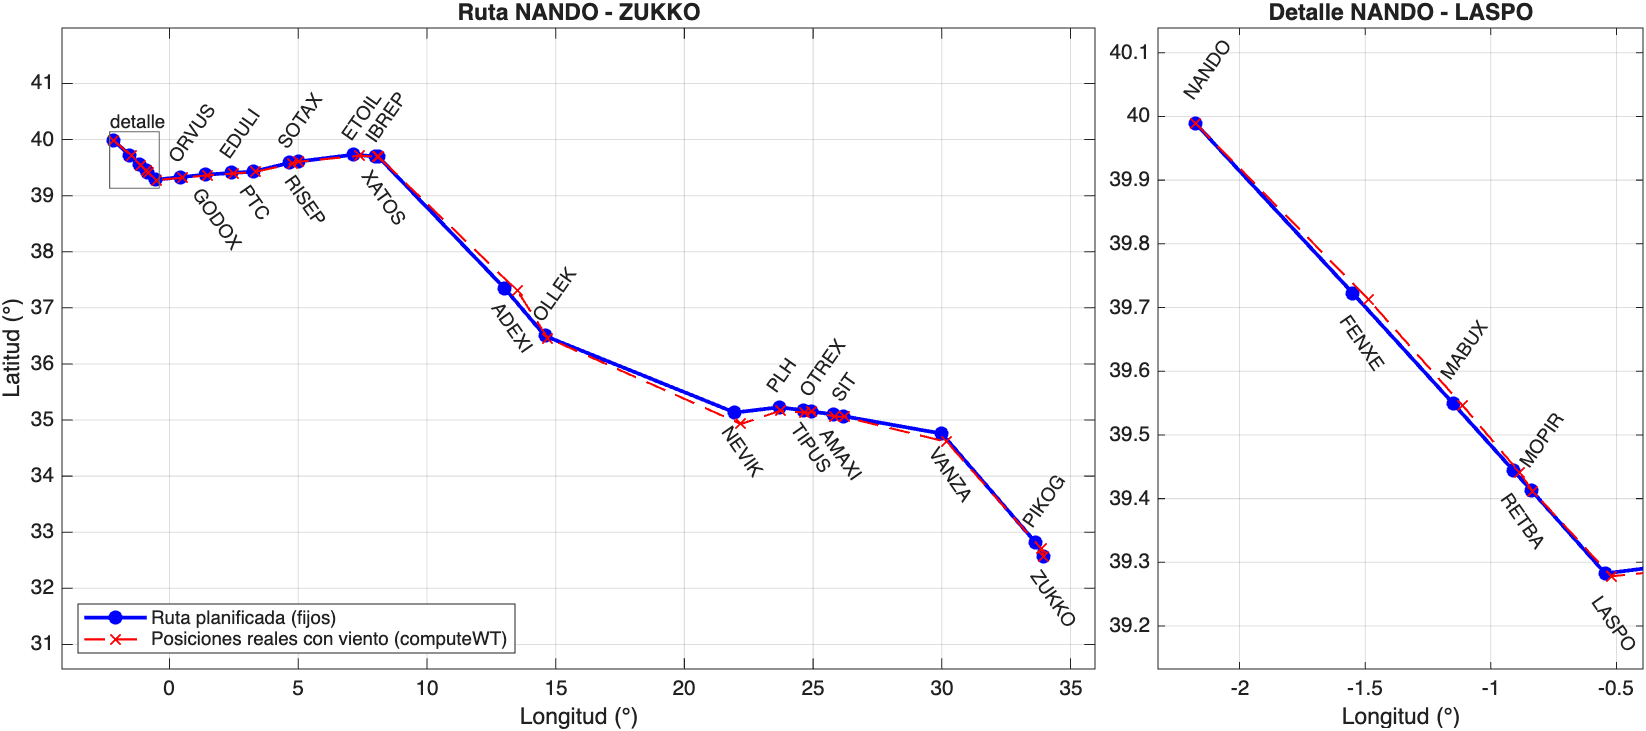
\includegraphics[width=\linewidth]{enroute-mapa.png}
\caption{Fase en-ruta: fijos planificados (azul) y posiciones reales alcanzadas al final de cada tramo volando a rumbo constante con el viento previsto (rojo), calculadas con \m{computeWT}; el panel derecho amplía el tramo NANDO--LASPO (recuadro gris del mapa). Las coordenadas son las de \m{enroute-sinviento.xlsx} y \m{enroute-conviento.kml}; la figura la genera \m{main\_enroute.m} (\m{plot\_enroute\_map}). La representación en Google Earth se entrega en los ficheros KML.}
\label{fig:mapa}
\end{figure}

\subsection{Límites de altitud de las rutas ATS}\label{sec:enr-pendiente}

El enunciado pide identificar cada ruta ATS volada y anotar sus límites de altitud en la tabla Excel. Las columnas «Altitud mínima/máxima» de \m{enroute-sinviento.xlsx} y \m{enroute-conviento.xlsx} están vacías (\m{NaN}) porque esos límites no se han podido comprobar en los AIP correspondientes; el código los admite como campos \m{alt\_min}/\m{alt\_max} de cada fijo (\m{main\_enroute.m}, líneas 13--17) y basta rellenarlos para que aparezcan en las tablas y en la comprobación del perfil vertical.

\pendiente{Los siguientes datos del en-ruta se han tomado del plan SimBrief (AIRAC \sbAirac) y \textbf{no} se han contrastado con un AIP: los fijos IBREP, ADEXI, OLLEK, NEVIK, PLH, TIPUS, OTREX, AMAXI, SIT, VANZA y PIKOG; las aerovías UL144 (NEVIK--PLH), UM978 (PLH--SIT) y L609 desde PIKOG hasta ZUKKO (en el AIP de Israel L609 solo figura desde KONFO); la descripción de los espacios de ruta libre de Italia, Grecia y Chipre que justifican los segmentos DCT IBREP--ADEXI--OLLEK--NEVIK y SIT--VANZA--PIKOG; y los límites de altitud (mínimo/máximo) de todas las rutas ATS del tramo, incluidas T257, UL144, UM978 y L609. Deben comprobarse en el AIP de Italia (ENAV, ENR 3 y ENR 4.4), Grecia (HCAA, ENR 3.3 / ruta libre), Chipre (ENR 3) e Israel (ENR 3.1 L609) y anotarse en las columnas de altitud de las tablas Excel. Están \textbf{verificados}: T257 y los fijos NANDO, FENXE, MABUX, RETBA, MOPIR, LASPO, ORVUS, GODOX, EDULI, PTC y SOTAX (AIP ENAIRE ENR 3.2 / ENR 4.4); SOTAX, RISEP, ETOIL y XATOS (AIP France ENR 4.4, espacio de ruta libre LFFRASE FL195--FL660); ZUKKO y KONFO (cartas de LLBG).}

\subsection{Tiempo de vuelo en condiciones de viento}\label{sec:viento}

\paragraph{Triángulo de velocidades.} El enunciado (sección~3.2) pide un tercer caso del triángulo de velocidades, distinto del cálculo clásico del ángulo de corrección de deriva: al inicio de cada tramo se fija un rumbo igual a la derrota deseada hacia el siguiente fijo, se mantiene ese rumbo durante el tiempo necesario para recorrer la distancia del tramo a la TAS de crucero y, al final, la posición real no coincide con el fijo por efecto del viento; el siguiente tramo parte de esa posición real. Conocidos el vector TAS (módulo $V$, rumbo $\psi$) y el vector viento (intensidad $w$, dirección de procedencia $\chi_w$), la incógnita es el vector GS:
\begin{equation}
\vec{V}_{GS} = \vec{V}_{TAS} + \vec{W} =
V\begin{pmatrix}\cos\psi\\ \sin\psi\end{pmatrix} + w\begin{pmatrix}\cos(\chi_w+180^\circ)\\ \sin(\chi_w+180^\circ)\end{pmatrix},\qquad
GS = \lVert\vec{V}_{GS}\rVert,\quad \chi = \operatorname{atan2}(V_{GS,E},\,V_{GS,N}),
\end{equation}
en componentes norte y este; se suman 180° a la dirección del viento porque el plan LIDO la da «desde». El tiempo del tramo es $t = d/V_{TAS}$, con $d$ la distancia ortodrómica desde la posición inicial real hasta el fijo, y el destino efectivo se obtiene avanzando $GS\cdot t$ sobre la derrota real $\chi$ con \m{orto\_reckon}. Esto es lo que hace \m{computeWT(lat1, lon1, lat2, lon2, windSpeed, windDir, tas)}, con la firma del enunciado más un séptimo argumento opcional (TAS, 450~kt por defecto). \m{route\_time\_wind} la llama iterativamente tramo a tramo, tomando como viento del tramo la previsión del fijo planificado en el que empieza (suposición~6, apéndice~\ref{ap:supuestos}), y rellena \m{tas}, \m{head}, \m{gs}, \m{track}, \m{dist}, \m{time} y las posiciones reales de \m{wp\_viento}.

\paragraph{Resultados.} La tabla~\ref{tab:enr1} reproduce \m{enroute-conviento.xlsx} ampliada con el rumbo, la desviación y el tiempo alternativo. El viento previsto es de componente oeste--noroeste (dirección 248°--328°, 21--47~kt), es decir, de cola en casi toda la ruta: la GS resultante está entre \enrGSmin{} y \enrGSmax~kt. Al volar cada tramo a rumbo constante el avión sobrepasa el fijo (desviación máxima \enrDevMax~NM al final del tramo IBREP--\enrDevMaxFix, el más largo), de modo que la suma de distancias desde las posiciones reales, \enrDistW~NM, es \enrDeltaD~NM menor que la planificada; al final del último tramo el avión queda a \enrDevZukko~NM de ZUKKO. El ángulo entre rumbo y derrota real no supera \enrWcaMax°.

\begingroup\scriptsize\setlength{\tabcolsep}{2.8pt}
\begin{longtable}{rlrrrrrrrr}
\caption{Fase en-ruta con viento (\texttt{enroute-conviento.xlsx}; rumbo, desviación y $t_{d/\mathrm{GS}}$ obtenidos con las mismas funciones). Cada tramo parte de la posición real alcanzada al final del anterior; $d$ es la distancia desde esa posición al siguiente fijo planificado y Desv.\ la distancia entre la posición real al final del tramo y el fijo. $t_{d/\mathrm{TAS}}$ es el criterio literal del enunciado (tiempo volado a rumbo constante); $t_{d/\mathrm{GS}}$ el criterio alternativo.}\label{tab:enr1}\\
\toprule
N.º & Fijo & Rumbo (°) & Derrota real (°) & GS (kt) & $d$ (NM) & $D$ (NM) & Desv. (NM) & $t_{d/\mathrm{TAS}}$ (s) & $t_{d/\mathrm{GS}}$ (s)\\
\midrule
\endfirsthead
\multicolumn{10}{l}{\small\itshape (continuación)}\\
\toprule
N.º & Fijo & Rumbo (°) & Derrota real (°) & GS (kt) & $d$ (NM) & $D$ (NM) & Desv. (NM) & $t_{d/\mathrm{TAS}}$ (s) & $t_{d/\mathrm{GS}}$ (s)\\
\midrule
\endhead
\midrule
\multicolumn{10}{r}{\small\itshape continúa}\\
\endfoot
\bottomrule
\endlastfoot
1 & NANDO & 0,0 & 0,0 & 450,0 & 0,00 & 0,00 & 0,00 & 0 & 0\\
2 & FENXE & 118,8 & 117,4 & 488,2 & 32,98 & 32,98 & 2,93 & 264 & 243\\
3 & MABUX & 122,1 & 119,9 & 489,0 & 18,41 & 51,39 & 1,76 & 411 & 379\\
4 & RETBA & 123,1 & 121,0 & 491,4 & 11,24 & 62,63 & 1,12 & 501 & 461\\
5 & MOPIR & 127,7 & 126,0 & 481,1 & 2,76 & 65,40 & 0,21 & 523 & 482\\
6 & LASPO & 119,9 & 118,8 & 482,6 & 15,50 & 80,89 & 1,17 & 647 & 597\\
7 & ORVUS & 85,5 & 86,7 & 482,5 & 44,31 & 125,20 & 3,35 & 1\,002 & 928\\
8 & GODOX & 85,3 & 86,5 & 482,7 & 42,35 & 167,55 & 3,20 & 1\,340 & 1\,244\\
9 & EDULI & 86,1 & 87,1 & 487,1 & 43,68 & 211,23 & 3,69 & 1\,690 & 1\,567\\
10 & PTC & 86,7 & 87,4 & 490,6 & 35,35 & 246,58 & 3,22 & 1\,973 & 1\,826\\
11 & SOTAX & 80,6 & 81,9 & 491,8 & 62,88 & 309,46 & 6,01 & 2\,476 & 2\,286\\
12 & RISEP & 78,1 & 79,7 & 495,2 & 9,33 & 318,78 & 0,97 & 2\,550 & 2\,354\\
13 & ETOIL & 84,9 & 85,9 & 496,3 & 99,62 & 418,40 & 10,40 & 3\,347 & 3\,077\\
14 & XATOS & 91,5 & 91,7 & 495,0 & 28,32 & 446,72 & 2,83 & 3\,574 & 3\,283\\
15 & IBREP & 90,8 & 91,0 & 489,0 & 2,25 & 448,97 & 0,19 & 3\,592 & 3\,299\\
16 & ADEXI & 119,9 & 117,8 & 485,1 & 270,33 & 719,30 & 23,42 & 5\,754 & 5\,305\\
17 & OLLEK & 132,8 & 131,4 & 483,3 & 70,59 & 789,89 & 5,49 & 6\,319 & 5\,831\\
18 & NEVIK & 100,5 & 101,9 & 468,0 & 362,86 & 1\,152,75 & 16,93 & 9\,222 & 8\,622\\
19 & PLH & 75,8 & 78,9 & 458,6 & 74,97 & 1\,227,72 & 4,33 & 9\,822 & 9\,211\\
20 & TIPUS & 89,1 & 92,3 & 469,6 & 44,62 & 1\,272,34 & 3,17 & 10\,179 & 9\,553\\
21 & OTREX & 83,8 & 86,7 & 469,0 & 13,08 & 1\,285,42 & 0,87 & 10\,283 & 9\,653\\
22 & AMAXI & 93,6 & 96,1 & 472,6 & 40,93 & 1\,326,35 & 2,73 & 10\,611 & 9\,965\\
23 & SIT & 89,2 & 91,7 & 473,6 & 18,09 & 1\,344,44 & 1,25 & 10\,756 & 10\,102\\
24 & VANZA & 94,4 & 96,6 & 475,2 & 187,54 & 1\,531,99 & 12,92 & 12\,256 & 11\,523\\
25 & PIKOG & 121,0 & 120,9 & 480,0 & 202,22 & 1\,734,20 & 13,48 & 13\,874 & 13\,040\\
26 & ZUKKO & 151,5 & 147,2 & 458,3 & 10,12 & 1\,744,32 & 0,79 & 13\,955 & 13\,119\\
\end{longtable}
\endgroup


\paragraph{Comparación y criterio de tiempo.} La tabla~\ref{tab:enrcomp} compara los tiempos. El enunciado define el tiempo de cada tramo como «el tiempo necesario para cubrir la distancia calculada a una velocidad de crucero de 450~kt», es decir $t=d/\mathrm{TAS}$; es el criterio adoptado en la columna «Tiempo total» de \m{enroute-conviento.xlsx} y da \enrTW{} (\enrTWh~h), \enrDiffW~min menos que sin viento solo porque las distancias desde las posiciones reales son menores. Como la lectura física habitual es que el avión recorre la distancia sobre el suelo a GS, el código calcula también $t=d/\mathrm{GS}$ (campo \m{time\_gs}), que da \enrTWg{} (\enrTWgh~h), \enrDiffWg~min menos que sin viento. Ambos valores se presentan; el criterio literal es el que figura en la tabla Excel, y la ambigüedad se consultará con el profesor.

\begin{table}[htbp]
\centering
\footnotesize\setlength{\tabcolsep}{3.5pt}
\caption{Comparación de los tiempos de la fase en-ruta (valores finales de las tablas \ref{tab:enr0} y \ref{tab:enr1}).}\label{tab:enrcomp}
\begin{tabular}{lrrr}
\toprule
 & Sin viento & Con viento, $t=d/\mathrm{TAS}$ & Con viento, $t=d/\mathrm{GS}$\\
\midrule
Distancia recorrida (NM) & 1\,852,1 & 1\,744,3 & 1\,744,3\\
Velocidad usada en el tiempo & TAS = 450 kt & TAS = 450 kt & GS (458--496 kt)\\
Tiempo NANDO--ZUKKO & 4:06:57 & 3:52:35 & 3:38:39\\
Tiempo (h) & 4,12 & 3,88 & 3,64\\
Diferencia respecto al caso sin viento (min) & -- & $-$14,4 & $-$28,3\\
\bottomrule
\end{tabular}
\end{table}


% ============================================================ 4
\Needspace{0.36\textheight}
\section{Fase de salida: SID NANDO3R (LEMD RWY 36R)}\label{sec:sid}

\subsection{Análisis de la carta}

La salida normalizada NANDO TRES ROMEO (NANDO3R, RNAV~1) de la pista 36R está en la carta AD~2-LEMD SID~7 del AIP ENAIRE. Su tabla de codificación es:

\begin{table}[H]\centering\small
\begin{tabular}{llllrll}\toprule
N.º & Tipo & Fijo & Derrota mag. (geo.) & Dist. (NM) & Altitud & IAS máx.\\ \midrule
001 & CA & -- & 360° & -- & +2\,500 ft & --\\
002 & CF & MD047 & 016° (015,3°) & -- & +3\,000 ft & 210 kt\\
003 & TF & MD048 & 041° (040,4°) & 12,6 & +7\,000 ft & 220 kt\\
004 & TF & MD049 & 128° (127,1°) & 5,0 & +8\,000 ft & --\\
005 & TF & MD824 & 158° (158,0°) & 19,4 & +13\,000 ft & 240 kt\\
006 & TF & MD922 & 139° (138,9°) & 21,5 & +13\,000 ft & --\\
007 & TF & NANDO (fly-over) & 107° (106,3°) & 30,4 & +13\,000 ft & --\\ \bottomrule
\end{tabular}
\caption{Codificación de la SID NANDO3R según la carta AD 2-LEMD SID 7 (AIP ENAIRE). «+» = a o por encima. La carta añade: «pendiente mínima de ascenso 5,5\,\% hasta MD824, debida a motivos operacionales» y «NANDO3R: sujeta a la actividad de la LED131».}
\label{tab:sidcarta}
\end{table}

Los fijos de la SID no aparecen en el plan SimBrief (que usa la NANDO6W, de un ciclo anterior), por lo que \m{main\_sid.m} los introduce directamente de la tabla de coordenadas de la carta (MD047 403537.1N 0033217.6W, MD048 404513.2N 0032133.3W, MD049 404212.4N 0031619.9W, MD824 402410.7N 0030649.4W, MD922 400758.5N 0024825.3W, NANDO 395919.9N 0021028.4W) mediante \m{build\_procedure} y \m{dms2deg}. El punto inicial es el extremo de pista DER 36R (403157.44N 0033333.77W, AD~2~LEMD). El tramo CA (ascenso en rumbo 360° hasta 2\,500~ft) no termina en un fijo: su final se ha calculado con \m{orto\_reckon} suponiendo que se alcanzan 2\,500~ft con la pendiente mínima del 5,5\,\% desde la elevación del aeródromo (1\,998~ft), lo que da el punto auxiliar CA2500 a \sidCA~NM del DER (suposición~1). No hay más curvas que requieran puntos auxiliares: el tramo CF a MD047 y los TF siguientes se representan como ortodrómicas entre fijos.

\subsection{Distancias y restricciones}

La tabla~\ref{tab:sid} reproduce \m{SID-NANDO3R.xlsx}. Las distancias calculadas (12,60; 4,98; 19,44; 21,46 y 30,32~NM) coinciden con las de la carta (12,6; 5,0; 19,4; 21,5 y 30,4~NM) dentro del redondeo, lo que valida las coordenadas introducidas; la longitud total DER--NANDO es \sidDist~NM. Las restricciones se calculan con \m{apply\_restrictions}:
\begin{itemize}
\item \emph{Altitud mínima} en cada fijo: el mayor de los dos valores entre el límite «a o por encima» de la carta y la altitud que resulta de ascender con la pendiente mínima del 5,5\,\% desde 1\,998~ft en el DER hasta MD824 ($h_{\min}=1998+0{,}055\,D$, con $D$ en ft). La pendiente resulta más restrictiva que la carta en todos los fijos hasta MD824: \sidMDOIVVIIalt~ft en MD047 (carta 3\,000), \sidMDOIVVIIIalt~ft en MD048 (7\,000), \sidMDOIVIXalt~ft en MD049 (8\,000) y \sidMDVIIIIIIValt~ft en MD824 (13\,000). A partir de MD824 la carta no impone pendiente y se mantiene la altitud mínima alcanzada (no se aplica el 3,3\,\% genérico, suposición~2). La columna «Pend.» confirma el 5,5\,\% en todos los tramos hasta MD824 y 0 después.
\item \emph{Altitud máxima}: la carta no da ninguna; se usa 40\,000~ft como valor «sin límite» (enunciado, sección~4).
\item \emph{IAS máxima}: la de la carta en MD047 (210~kt), MD048 (220~kt) y MD824 (240~kt); 250~kt por debajo de 10\,000~ft en los fijos sin límite propio (DER, CA2500, MD049); 350~kt («sin límite») por encima de 10\,000~ft (MD922, NANDO). No hay IAS mínimas en la carta.
\end{itemize}

\begingroup\scriptsize\setlength{\tabcolsep}{2.8pt}
\begin{longtable}{rlrrrrrrrrr>{\raggedright\arraybackslash}p{3.4cm}}
\caption{SID NANDO3R desde el DER 36R (\texttt{SID-NANDO3R.xlsx}). Alt mín = máx(límite «a o por encima» de la carta, altitud de la pendiente mínima del 5,5\,\% desde 1998 ft hasta MD824); IAS máx = límite de la carta, 250 kt por debajo de 10\,000 ft o 350 kt (sin límite). $D$: distancia acumulada desde el DER; Pend.: pendiente mínima del tramo deducida de las altitudes mínimas.}\label{tab:sid}\\
\toprule
N.º & Fijo & Lat (°) & Lon (°) & \makecell{Alt mín\\(ft)} & \makecell{Alt máx\\(ft)} & \makecell{IAS máx\\(kt)} & \makecell{Derrota\\(°)} & \makecell{$d$\\(NM)} & \makecell{$D$\\(NM)} & \makecell{Pend.\\(\%)} & Descripción (carta)\\
\midrule
\endfirsthead
\multicolumn{12}{l}{\small\itshape (continuación)}\\
\toprule
N.º & Fijo & Lat (°) & Lon (°) & \makecell{Alt mín\\(ft)} & \makecell{Alt máx\\(ft)} & \makecell{IAS máx\\(kt)} & \makecell{Derrota\\(°)} & \makecell{$d$\\(NM)} & \makecell{$D$\\(NM)} & \makecell{Pend.\\(\%)} & Descripción (carta)\\
\midrule
\endhead
\midrule
\multicolumn{12}{r}{\small\itshape continúa}\\
\endfoot
\bottomrule
\endlastfoot
1 & DER36R & 40,5326 & $-$3,5594 & 1\,998 & 40\,000 & 250 & 0,0 & 0,00 & 0,00 & -- & \scriptsize End of RWY 36R (AD 2 LEMD)\\
2 & CA2500 & 40,5576 & $-$3,5594 & 2\,500 & 40\,000 & 250 & 0,0 & 1,50 & 1,50 & 5,50 & \scriptsize CA leg 360 to 2500 ft (position computed, see below)\\
3 & MD047 & 40,5936 & $-$3,5382 & 3\,291 & 40\,000 & 210 & 24,1 & 2,37 & 3,87 & 5,50 & \scriptsize CF 015.3\\
4 & MD048 & 40,7537 & $-$3,3592 & 7\,501 & 40\,000 & 220 & 40,2 & 12,60 & 16,47 & 5,50 & \scriptsize TF 040.4\\
5 & MD049 & 40,7034 & $-$3,2722 & 9\,165 & 40\,000 & 250 & 127,3 & 4,98 & 21,45 & 5,50 & \scriptsize TF 127.1\\
6 & MD824 & 40,4030 & $-$3,1137 & 15\,660 & 40\,000 & 240 & 158,1 & 19,44 & 40,88 & 5,50 & \scriptsize TF 158.0 (end of 5.5\% min gradient)\\
7 & MD922 & 40,1329 & $-$2,8070 & 15\,660 & 40\,000 & 350 & 139,0 & 21,46 & 62,34 & 0,00 & \scriptsize TF 138.9\\
8 & NANDO & 39,9889 & $-$2,1746 & 15\,660 & 40\,000 & 350 & 106,4 & 30,32 & 92,66 & 0,00 & \scriptsize TF 106.3, fly-over\\
\end{longtable}
\endgroup


\begin{figure}[!htbp]\centering
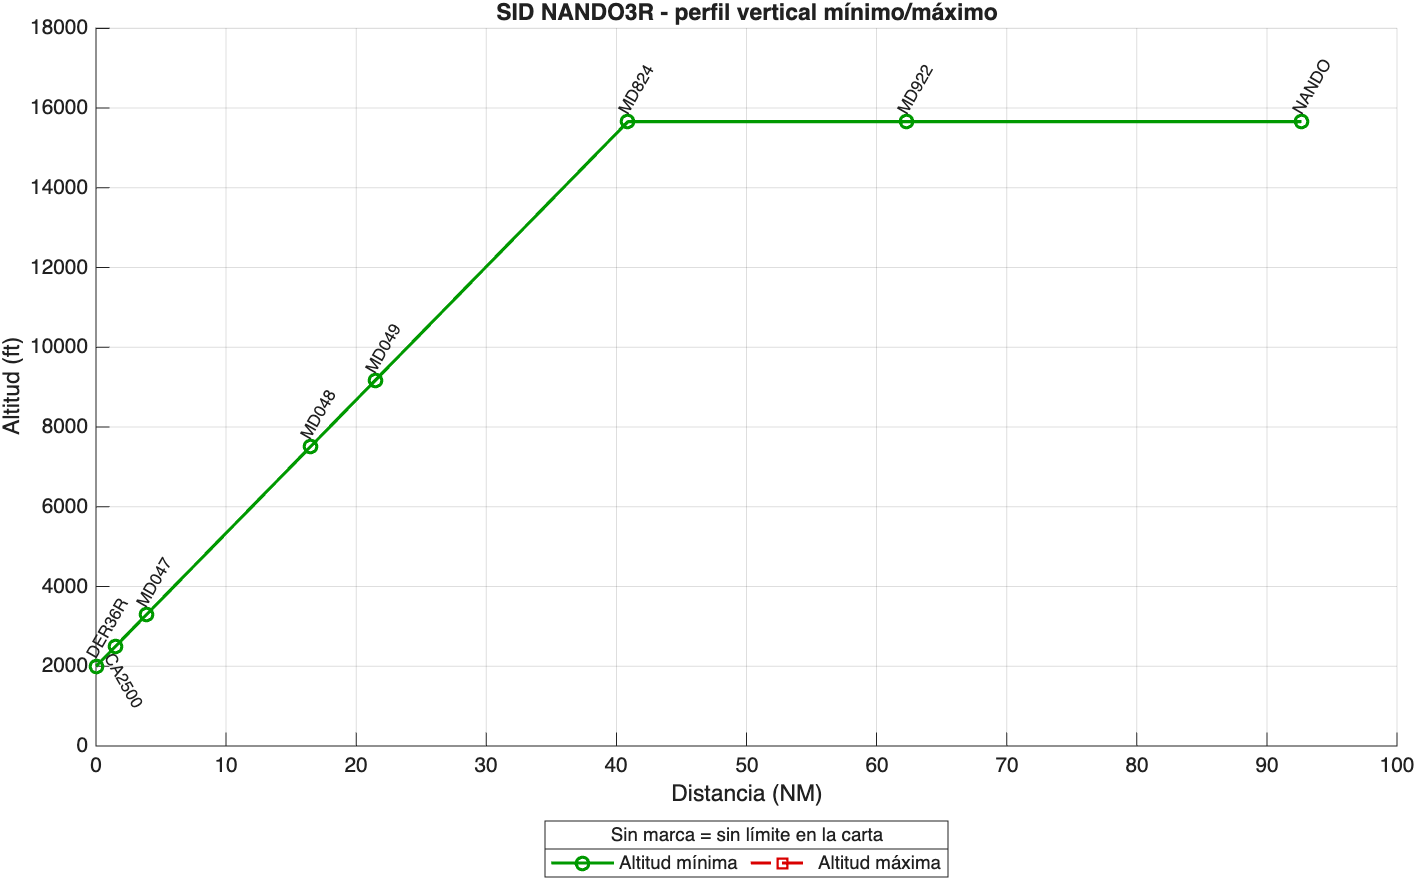
\includegraphics[width=0.9\linewidth]{SID-NANDO3R-vertical.png}
\caption{SID NANDO3R: altitud mínima y máxima en cada fijo frente a la distancia acumulada desde el DER 36R (\m{SID-NANDO3R-vertical.png}). La carta no da altitudes máximas: el valor «sin límite» (40\,000 ft) no se dibuja.}
\label{fig:sidv}
\end{figure}

\paragraph{Atenuación de ruido.} LEMD AD~2.21 (AIP ENAIRE) prescribe para el despegue: hasta 450~m (1\,500~ft) sobre el aeródromo, potencia y flaps de despegue y V$_2$+10 a 20~kt; a 1\,500~ft reducir a no menos de la potencia de ascenso; de 1\,500 a 3\,000~ft mantener V$_2$+10 a 20~kt; a 3\,000~ft acelerar gradualmente a la velocidad de ascenso retrayendo flaps. Estos tramos definen C1, C2 y C3 del perfil vertical (sección~\ref{sec:vertical}). El B738 no está en la lista de tipos a los que LEMD impone las SID «X» de la 36L.

% ============================================================ 5
\section{Fases de llegada y aproximación (LLBG RWY 21)}\label{sec:llegada}

Las tres fases se resuelven en \m{main\_star\_app.m}: la transición ERREZ1A desde ZUKKO hasta TOPPU, la aproximación ILS~21 desde TOPPU (precisión), su frustrada y la aproximación RNP~Y~21 desde TOPPU (no precisión). Todas las coordenadas se toman de las tablas de las cartas del eAIP de Israel y se introducen con \m{build\_procedure}; \m{route\_distances} calcula las distancias voladas, \m{to\_remaining\_dist} las convierte en distancia restante hasta THR21 y \m{apply\_chart\_limits} asigna los límites de altitud e IAS de las cartas (sin pendiente mínima, que las cartas no imponen). Los KML son \m{LEMD-LLBG-llegada.kml}, \m{LEMD-LLBG-apr-ILS21.kml}, \m{LEMD-LLBG-frustrada-ILS21.kml} y \m{LEMD-LLBG-apr-RNPY21.kml}.

\subsection{Llegada: transición ERREZ1A (ZUKKO a TOPPU)}

ZUKKO es el punto final del en-ruta (L609) y el IF de la transición ERREZ1A a las pistas 21/26 (carta AD~2 LLBG TRANS 21-26, 18 MAY 23); es también el IF de las STAR AMMOS1A/1B de la carta STAR 21-26, que no se vuelan. La codificación de la carta es:

\begin{table}[H]\centering\small
\begin{tabular}{lllrlll}\toprule
Tipo & Fijo & Derrota (T) & Dist. (NM) & Viraje & Altitud & IAS máx.\\ \midrule
IF & ZUKKO & -- & -- & -- & $-$13\,000 & --\\
TF & KONFO & 133,4° & 11,6 & -- & +10\,000 / $-$11\,000 & --\\
TF & ERREZ & 071,5° & 23,2 & izq. & @9\,000 & --\\
TF & IVONA & 071,8° & 9,8 & -- & @9\,000 & --\\
TF & RAPIV & 094,9° & 10,1 & der. & @9\,000 & --\\
TF & ALIQA & 094,9° & 5,0 & -- & @9\,000 & 250 kt\\
TF & LEGOH & 094,9° & 11,5 & -- & @9\,000 & 250 kt\\
TF & ANOZA & 209,0° & 18,3 & der. & +5\,000 & 250 kt\\
TF & TOPPU & 209,0° & 3,1 & -- & +4\,000 & 250 kt\\ \bottomrule
\end{tabular}
\caption{Codificación de la transición ERREZ1A (AD 2 LLBG TRANS 21-26). «@» = a; «+» = a o por encima; «$-$» = a o por debajo. Desde TOPPU: «seguir instrucciones ATC»; fallo de comunicaciones: «desde TOPPU descender a 2\,600 ft hacia GALGA e interceptar el ILS RWY 21».}
\label{tab:transcarta}
\end{table}

La tabla~\ref{tab:llegada} reproduce \m{LLEGADA-ERREZ1A.xlsx}. Las distancias calculadas (11,62; 23,19; 9,77; 10,07; 4,99; 11,46; 18,32 y 3,10~NM) coinciden con la carta; la transición mide \arrDist~NM y TOPPU queda a \arrToppuRest~NM del umbral por la ILS. Los límites se codifican así: ZUKKO máximo 13\,000~ft (sin mínimo); KONFO ventana 10\,000--11\,000~ft; ERREZ a LEGOH exactamente 9\,000~ft (mínimo = máximo); ANOZA y TOPPU mínimos de 5\,000 y 4\,000~ft; IAS máxima 250~kt desde ALIQA (carta) y en todos los fijos por debajo de 10\,000~ft; en ZUKKO y KONFO no hay límite de IAS en la carta y, al estar a 10\,000~ft o más, se deja en 350~kt («sin límite»). La figura~\ref{fig:llegv} muestra los límites verticales.

\paragraph{Esperas y transición al IF.} La carta publica esperas de 1~min en ZUKKO, KONFO (virajes a la derecha) y ERREZ (izquierda); no hay trombón ni \emph{point merge} que permitan acortar la ruta, de modo que la trayectoria nominal es la más larga posible: se vuelan todos los fijos y no se modelan las esperas (suposición~7). El enlace entre el final de la transición (TOPPU) y el IF de la ILS (GALGA) no está codificado («follow ATC instructions»); se ha adoptado el procedimiento de fallo de comunicaciones de la propia carta, TOPPU $\rightarrow$ GALGA directo a 2\,600~ft (suposición~4), que es \ilsGalgaLeg~NM en derrota 208,8°, prácticamente alineado con el localizador.

\begingroup\scriptsize\setlength{\tabcolsep}{2.8pt}
\begin{longtable}{rlrrrrrrrr>{\raggedright\arraybackslash}p{3.4cm}}
\caption{Transición ERREZ1A de ZUKKO a TOPPU (\texttt{LLEGADA-ERREZ1A.xlsx}). $D_{\mathrm{rest}}$: distancia restante hasta THR 21 por la ILS 21. «@9000» en la carta se codifica como mínimo = máximo = 9000 ft; 40\,000 ft y 350 kt indican ausencia de límite.}\label{tab:llegada}\\
\toprule
N.º & Fijo & Lat (°) & Lon (°) & \makecell{Alt mín\\(ft)} & \makecell{Alt máx\\(ft)} & \makecell{IAS máx\\(kt)} & \makecell{Derrota\\(°)} & \makecell{$d$\\(NM)} & \makecell{$D_{\mathrm{rest}}$\\(NM)} & Descripción (carta)\\
\midrule
\endfirsthead
\multicolumn{11}{l}{\small\itshape (continuación)}\\
\toprule
N.º & Fijo & Lat (°) & Lon (°) & \makecell{Alt mín\\(ft)} & \makecell{Alt máx\\(ft)} & \makecell{IAS máx\\(kt)} & \makecell{Derrota\\(°)} & \makecell{$d$\\(NM)} & \makecell{$D_{\mathrm{rest}}$\\(NM)} & Descripción (carta)\\
\midrule
\endhead
\midrule
\multicolumn{11}{r}{\small\itshape continúa}\\
\endfoot
\bottomrule
\endlastfoot
1 & ZUKKO & 32,5617 & 33,9492 & 0 & 13\,000 & 350 & 0,0 & 0,00 & 108,55 & \scriptsize IF, inicio de la ERREZ1A (máx. 13000)\\
2 & KONFO & 32,4283 & 34,1156 & 10\,000 & 11\,000 & 350 & 133,5 & 11,62 & 96,92 & \scriptsize TF 133,4T (10000-11000)\\
3 & ERREZ & 32,5503 & 34,5500 & 9\,000 & 9\,000 & 250 & 71,5 & 23,19 & 73,74 & \scriptsize TF 071,5T, viraje a la izquierda (@9000)\\
4 & IVONA & 32,6012 & 34,7333 & 9\,000 & 9\,000 & 250 & 71,7 & 9,77 & 63,97 & \scriptsize TF 071,8T (@9000)\\
5 & RAPIV & 32,5867 & 34,9317 & 9\,000 & 9\,000 & 250 & 94,9 & 10,07 & 53,90 & \scriptsize TF 094,9T, viraje a la derecha (@9000)\\
6 & ALIQA & 32,5805 & 35,0300 & 9\,000 & 9\,000 & 250 & 94,2 & 4,99 & 48,91 & \scriptsize TF 094,9T (@9000, máx. 250)\\
7 & LEGOH & 32,5647 & 35,2557 & 9\,000 & 9\,000 & 250 & 94,7 & 11,46 & 37,45 & \scriptsize TF 094,9T (@9000, máx. 250)\\
8 & ANOZA & 32,2975 & 35,0812 & 5\,000 & 40\,000 & 250 & 208,9 & 18,32 & 19,13 & \scriptsize TF 209,0T, viraje a la derecha (mín. 5000)\\
9 & TOPPU & 32,2522 & 35,0518 & 4\,000 & 40\,000 & 250 & 208,7 & 3,10 & 16,03 & \scriptsize TF 209,0T (mín. 4000); luego ATC (fallo de com.: directo a GALGA)\\
\end{longtable}
\endgroup


\begin{figure}[!htbp]\centering
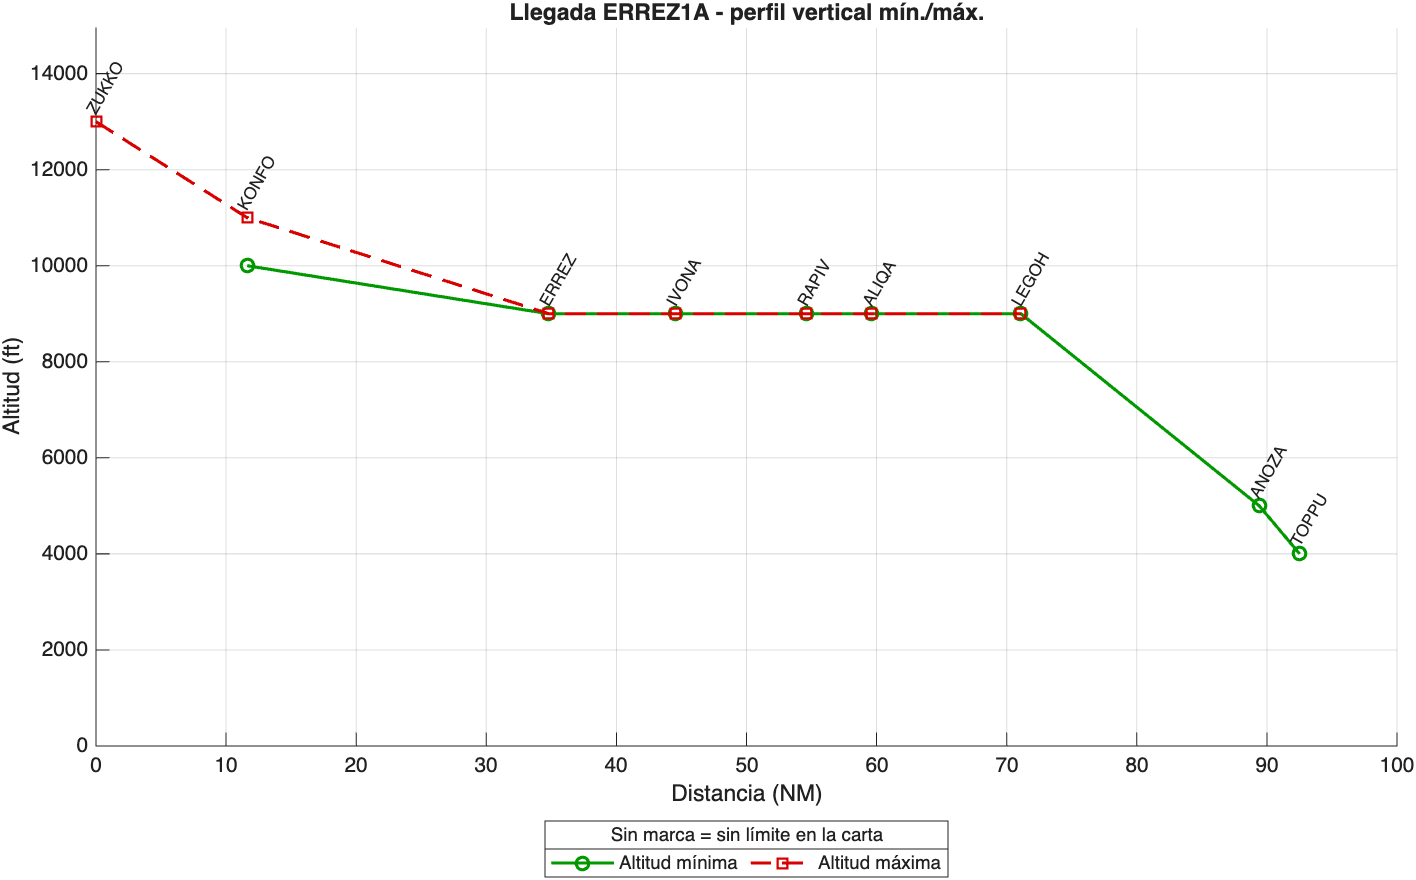
\includegraphics[width=0.85\linewidth]{LLEGADA-vertical.png}
\caption{Transición ERREZ1A: altitud mínima y máxima en cada fijo frente a la distancia volada desde ZUKKO (\m{LLEGADA-vertical.png}). ZUKKO no tiene altitud mínima en la carta: solo se dibuja su máxima (13\,000~ft).}
\label{fig:llegv}
\end{figure}

\subsection{Aproximación de precisión: ILS RWY 21}

Carta AD~2 LLBG IAC-21ILS-4 (31 OCT 24). Fijos y codificación relevantes para nuestra ruta: GALGA (IF, 320925N 0345924E, +2\,600~ft), BG074 (FAP, 320736.81N 0345813.95E, 2,1~NM de GALGA, 7,4~DME BN, +2\,600~ft), THR21 (320105.25N 0345400.81E, 7,4~NM del FAP). Senda de planeo 3,0°, RDH 50~ft, elevación del umbral 134~ft; la altitud de cruce del umbral que figura en la tabla de la carta, 183~ft (134 + 50 ~ft, más el redondeo de la carta), es la que se usa como altitud del punto THR21. OCA(H) ILS CAT~I para categoría C: 313~ft (179~ft). La tabla~\ref{tab:ils} reproduce \m{APR-ILS21.xlsx}: GALGA--BG074 \ilsFapLeg~NM y BG074--THR21 \ilsFinal~NM, iguales a la carta; la pendiente media entre 2\,600 y 183~ft en \ilsFinal~NM es \ilsGPdeg°, coherente con la senda de 3°. La aproximación intermedia es GALGA--BG074 a 2\,600~ft; la final, desde el FAP; la IAS máxima en los fijos (250~kt bajo 10\,000~ft) es la genérica, ya que la carta solo limita la velocidad en el segmento inicial (230/220~kt, no volado) y en la frustrada (190~kt).

\begingroup\scriptsize\setlength{\tabcolsep}{2.8pt}
\begin{longtable}{rlrrrrrrrr>{\raggedright\arraybackslash}p{3.4cm}}
\caption{Aproximación de precisión ILS RWY 21 desde TOPPU (\texttt{APR-ILS21.xlsx}).}\label{tab:ils}\\
\toprule
N.º & Fijo & Lat (°) & Lon (°) & \makecell{Alt mín\\(ft)} & \makecell{Alt máx\\(ft)} & \makecell{IAS máx\\(kt)} & \makecell{Derrota\\(°)} & \makecell{$d$\\(NM)} & \makecell{$D_{\mathrm{rest}}$\\(NM)} & Descripción (carta)\\
\midrule
\endfirsthead
\multicolumn{11}{l}{\small\itshape (continuación)}\\
\toprule
N.º & Fijo & Lat (°) & Lon (°) & \makecell{Alt mín\\(ft)} & \makecell{Alt máx\\(ft)} & \makecell{IAS máx\\(kt)} & \makecell{Derrota\\(°)} & \makecell{$d$\\(NM)} & \makecell{$D_{\mathrm{rest}}$\\(NM)} & Descripción (carta)\\
\midrule
\endhead
\midrule
\multicolumn{11}{r}{\small\itshape continúa}\\
\endfoot
\bottomrule
\endlastfoot
1 & TOPPU & 32,2522 & 35,0518 & 4\,000 & 40\,000 & 250 & 208,7 & 3,10 & 16,03 & \scriptsize TF 209.0T (min 4000); then ATC / comm failure: direct GALGA\\
2 & GALGA & 32,1569 & 34,9900 & 2\,600 & 40\,000 & 250 & 208,8 & 6,52 & 9,50 & \scriptsize IF ILS 21 (min 2600)\\
3 & BG074 & 32,1269 & 34,9705 & 2\,600 & 40\,000 & 250 & 208,7 & 2,06 & 7,45 & \scriptsize FAP ILS 21 (7.4 DME BN)\\
4 & THR21 & 32,0181 & 34,9002 & 183 & 40\,000 & 250 & 208,7 & 7,45 & 0,00 & \scriptsize RWY 21 threshold\\
\end{longtable}
\endgroup


\begin{figure}[!htbp]\centering
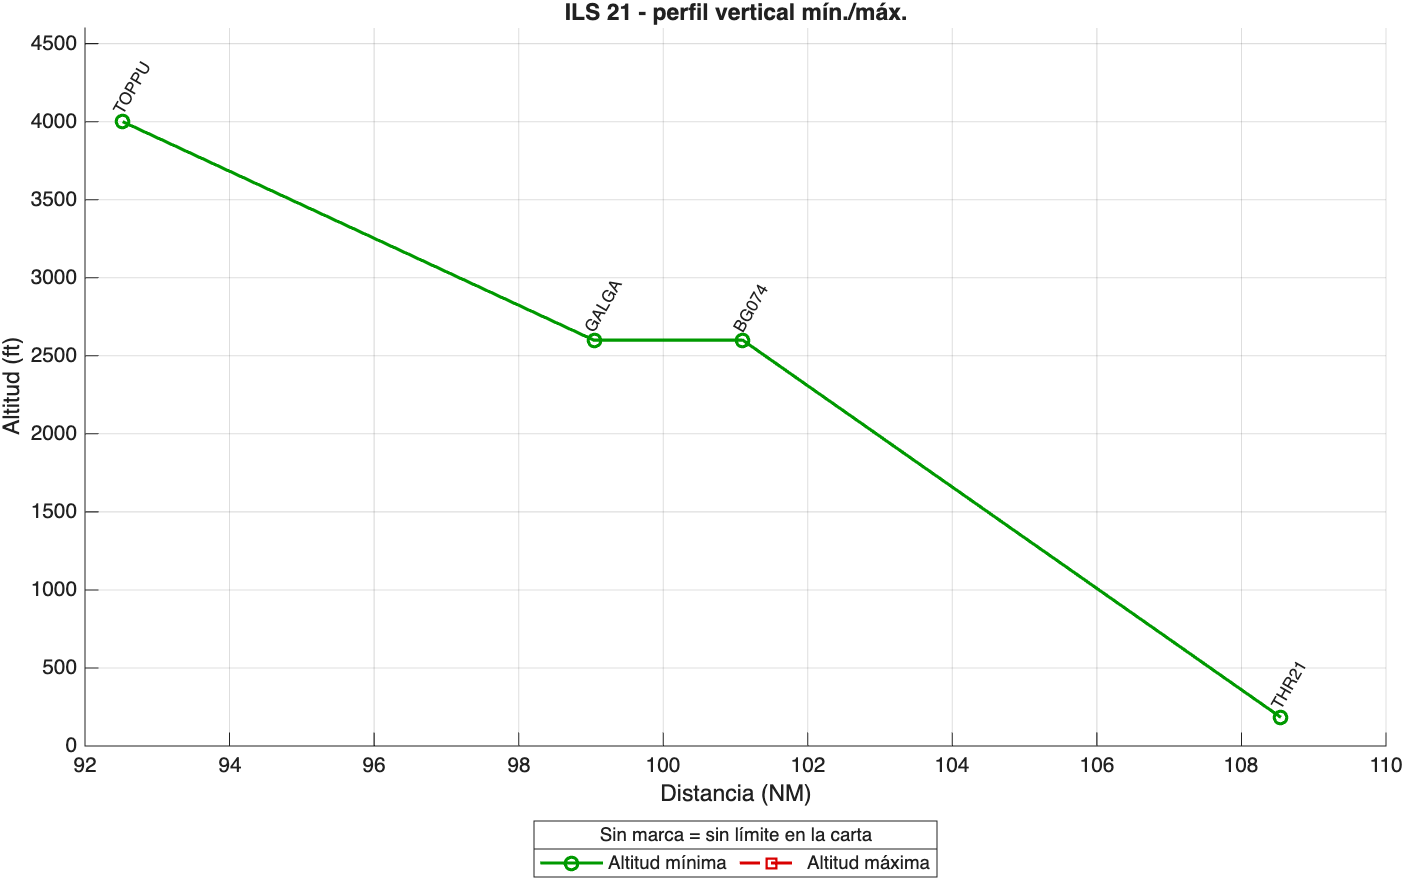
\includegraphics[width=0.8\linewidth]{APR-ILS21-vertical.png}
\caption{Aproximación ILS 21 desde TOPPU: altitudes mínima y máxima frente a la distancia volada (\m{APR-ILS21-vertical.png}).}
\end{figure}

\paragraph{Aproximación frustrada.} Según la carta: «Initial climb 5\,000. Climb on course 204°. Upon reaching 1\,000 turn LEFT (MAX 190 KIAS) to GEMDA 5\,000 and HOLD. Missed approach requires a 4.5\,\% (270 ft/NM) climb gradient due to airspace restrictions». Se ha modelado como el tramo THR21 (MAPt) $\rightarrow$ GEMDA (320326N 0345948E, a 5\,000~ft, IAS máx. 190~kt) en \m{LEMD-LLBG-frustrada-ILS21.kml} y \m{FRUSTRADA-ILS21.xlsx} (tabla~\ref{tab:frustrada}); su longitud ortodrómica es \misDist~NM. Es una simplificación: la trayectoria real sigue el rumbo 204° hasta 1\,000~ft (unas 3,2~NM desde la elevación de la pista al 4,5\,\%) y vira después a la izquierda hacia GEMDA (suposición~17 y apéndice~\ref{ap:otra-ruta}).

\begingroup\scriptsize\setlength{\tabcolsep}{2.8pt}
\begin{longtable}{rlrrrrrrrrr>{\raggedright\arraybackslash}p{3.4cm}}
\caption{Aproximación frustrada ILS RWY 21 (\texttt{FRUSTRADA-ILS21.xlsx}), común a la RNP Y 21. $D$: distancia acumulada desde THR21. Se modela solo el tramo THR21 $\rightarrow$ GEMDA (suposición~17).}\label{tab:frustrada}\\
\toprule
N.º & Fijo & Lat (°) & Lon (°) & \makecell{Alt mín\\(ft)} & \makecell{Alt máx\\(ft)} & \makecell{IAS máx\\(kt)} & \makecell{Derrota\\(°)} & \makecell{$d$\\(NM)} & \makecell{$D$\\(NM)} & \makecell{Pend.\\(\%)} & Descripción (carta)\\
\midrule
\endfirsthead
\multicolumn{12}{l}{\small\itshape (continuación)}\\
\toprule
N.º & Fijo & Lat (°) & Lon (°) & \makecell{Alt mín\\(ft)} & \makecell{Alt máx\\(ft)} & \makecell{IAS máx\\(kt)} & \makecell{Derrota\\(°)} & \makecell{$d$\\(NM)} & \makecell{$D$\\(NM)} & \makecell{Pend.\\(\%)} & Descripción (carta)\\
\midrule
\endhead
\midrule
\multicolumn{12}{r}{\small\itshape continúa}\\
\endfoot
\bottomrule
\endlastfoot
1 & THR21 & 32,0181 & 34,9002 & 183 & 40\,000 & 250 & 0,0 & 0,00 & 0,00 & -- & \scriptsize MAPt\\
2 & GEMDA & 32,0572 & 34,9967 & 5\,000 & 5\,000 & 190 & 64,4 & 5,44 & 5,44 & -- & \scriptsize DF, missed approach, @5000\\
\end{longtable}
\endgroup


\subsection{Aproximación de no precisión: RNP Y RWY 21}

Carta AD~2 LLBG IAC 21RNPY-3 (06 AUG 2026, AIRAC AMDT 001/2026), «RNP APCH, RF required». A diferencia de la LOC~21, su recorrido lateral es distinto del de la ILS: entra por el IAF GINTU (320448N 0350958E), al sureste del aeropuerto, y describe un giro hacia el norte y luego hacia el sur hasta alinearse con la pista mediante un tramo RF. Codificación:

\begin{table}[H]\centering\small
\begin{tabular}{lllrll}\toprule
Tipo & Fijo & Derrota (T) & Dist. (NM) & Altitud & IAS máx.\\ \midrule
IAF & GINTU & -- & -- & +6\,000 & --\\
TF & RABIN & 320,8° & 3,5 & +4\,000 & --\\
TF & OFFIK & 305,7° & 6,8 & +3\,500 & --\\
TF & VATAT & 290,7° & 4,1 & +3\,500 & 210 kt\\
TF & NAMIM (IF) & 180,9° & 3,8 & +2\,500 & 185 kt\\
TF & BG217 & 179,5° & 4,2 & +1\,200 & 185 kt\\
RF & BG216 (FAF) & arco a la derecha, $r$ = 2,55 NM & 1,3 & +1\,200 & 185 kt\\
TF & THR21 (MAPt) & 208,8° & 3,1 & +183 & 190 kt\\ \bottomrule
\end{tabular}
\caption{Codificación de la RNP Y RWY 21 (AD 2 LLBG IAC 21RNPY-3). Centro del arco RF: BG999 (320504.6N 0345310.0E). VPA 3,0° (Baro-VNAV: temperatura $-$10/+60~°C; VPA efectivo 2,8° a 0~°C y 3,3° a 45~°C). Frustrada idéntica a la de la ILS 21 (ascenso inicial a 5\,000 ft en rumbo 204°, a 1\,000 ft viraje a la izquierda, máx. 190 kt, a GEMDA).}
\label{tab:rnpcarta}
\end{table}

\paragraph{Enlace TOPPU $\rightarrow$ GINTU.} No está publicado ningún tramo desde el final de la transición hasta el IAF de la RNP~Y: se supone una instrucción ATC «directo GINTU» (suposición~5), de \rnpGintuLeg~NM. Se ha elegido GINTU, y no una entrada por NAMIM (IF), porque es el IAF publicado y da la trayectoria más larga, como pide el enunciado para los patrones de transición.

\paragraph{Puntos auxiliares del arco RF.} El tramo BG217 $\rightarrow$ BG216 es un arco de radio 2,55~NM centrado en BG999 con viraje a la derecha. La función \m{add\_arc\_points} calcula las marcaciones del centro a BG217 y a BG216 con \m{orto\_distazi} y genera puntos intermedios cada 10° con \m{orto\_reckon} (ARC1 y ARC2, marcaciones 100° y 110° desde el centro), heredando los límites del arco (+1\,200~ft, 185~kt). La longitud poligonal resultante BG217--ARC1--ARC2--BG216 es \rnpArc~NM, frente a 1,3~NM en la carta. La tabla~\ref{tab:rnp} reproduce \m{APR-RNPY21.xlsx}: las distancias de los tramos rectos (3,52; 6,83; 4,15; 3,75; 4,19 y \rnpFinal~NM) coinciden con la carta y la aproximación mide \rnpDist~NM desde TOPPU (frente a \arrToppuRest~NM por la ILS). Los límites de IAS de VATAT (210~kt), NAMIM, BG217, BG216 (185~kt) y THR21 (190~kt, frustrada) son los de la carta; los demás fijos llevan el genérico de 250~kt.

\begingroup\scriptsize\setlength{\tabcolsep}{2.8pt}
\begin{longtable}{rlrrrrrrrr>{\raggedright\arraybackslash}p{3.4cm}}
\caption{Aproximación de no precisión RNP Y RWY 21 desde TOPPU (\texttt{APR-RNPY21.xlsx}). ARC1 y ARC2 son puntos auxiliares del arco RF BG217--BG216 (centro BG999, radio 2,55 NM, paso 10°).}\label{tab:rnp}\\
\toprule
N.º & Fijo & Lat (°) & Lon (°) & \makecell{Alt mín\\(ft)} & \makecell{Alt máx\\(ft)} & \makecell{IAS máx\\(kt)} & \makecell{Derrota\\(°)} & \makecell{$d$\\(NM)} & \makecell{$D_{\mathrm{rest}}$\\(NM)} & Descripción (carta)\\
\midrule
\endfirsthead
\multicolumn{11}{l}{\small\itshape (continuación)}\\
\toprule
N.º & Fijo & Lat (°) & Lon (°) & \makecell{Alt mín\\(ft)} & \makecell{Alt máx\\(ft)} & \makecell{IAS máx\\(kt)} & \makecell{Derrota\\(°)} & \makecell{$d$\\(NM)} & \makecell{$D_{\mathrm{rest}}$\\(NM)} & Descripción (carta)\\
\midrule
\endhead
\midrule
\multicolumn{11}{r}{\small\itshape continúa}\\
\endfoot
\bottomrule
\endlastfoot
1 & TOPPU & 32,2522 & 35,0518 & 4\,000 & 40\,000 & 250 & 0,0 & 0,00 & 38,73 & \scriptsize TF 209.0T (min 4000); then ATC / comm failure: direct GALGA\\
2 & GINTU & 32,0800 & 35,1661 & 6\,000 & 40\,000 & 250 & 150,6 & 11,86 & 26,87 & \scriptsize IAF RNP Y 21 (link from TOPPU by ATC, assumed)\\
3 & RABIN & 32,1256 & 35,1225 & 4\,000 & 40\,000 & 250 & 321,0 & 3,52 & 23,35 & \scriptsize TF 320.8T\\
4 & OFFIK & 32,1921 & 35,0134 & 3\,500 & 40\,000 & 250 & 305,8 & 6,83 & 16,52 & \scriptsize TF 305.7T\\
5 & VATAT & 32,2167 & 34,9369 & 3\,500 & 40\,000 & 210 & 290,8 & 4,15 & 12,36 & \scriptsize TF 290.7T\\
6 & NAMIM & 32,1542 & 34,9358 & 2\,500 & 40\,000 & 185 & 180,9 & 3,75 & 8,61 & \scriptsize IF, TF 180.9T\\
7 & BG217 & 32,0844 & 34,9361 & 1\,200 & 40\,000 & 185 & 179,8 & 4,19 & 4,42 & \scriptsize TF 179.5T\\
8 & ARC1 & 32,0770 & 34,9354 & 1\,200 & 40\,000 & 185 & 184,5 & 0,44 & 3,98 & \scriptsize RF arc aux, brg 100 from centre\\
9 & ARC2 & 32,0699 & 34,9331 & 1\,200 & 40\,000 & 185 & 195,3 & 0,44 & 3,53 & \scriptsize RF arc aux, brg 110 from centre\\
10 & BG216 & 32,0641 & 34,9299 & 1\,200 & 40\,000 & 185 & 205,1 & 0,38 & 3,15 & \scriptsize FAF, RF arc r=2.55 NM, right\\
11 & THR21 & 32,0181 & 34,9002 & 183 & 40\,000 & 190 & 208,7 & 3,15 & 0,00 & \scriptsize MAPt, TF 208.8T\\
\end{longtable}
\endgroup


\begin{figure}[!htbp]\centering
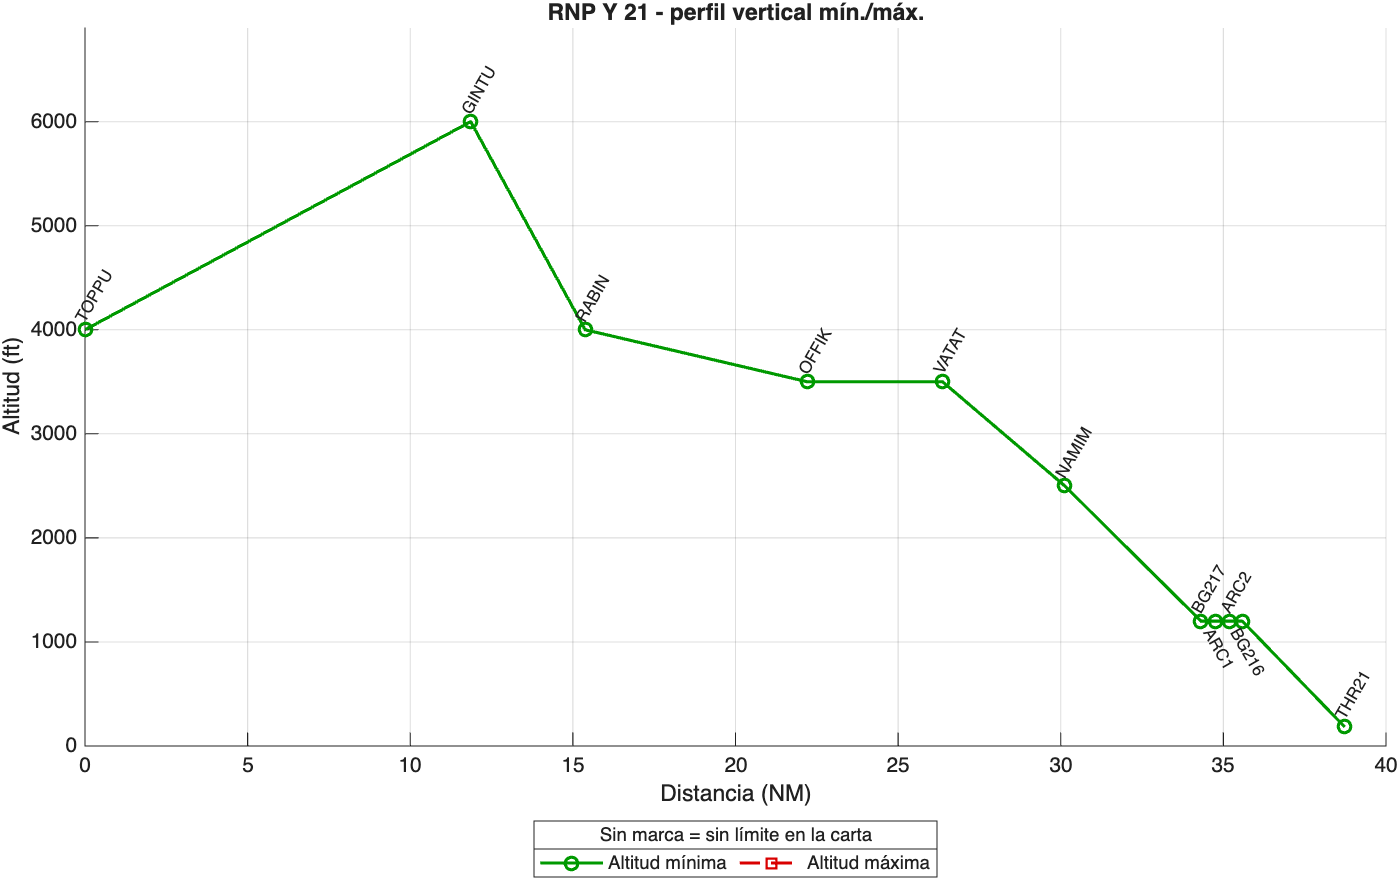
\includegraphics[width=0.8\linewidth]{APR-RNPY21-vertical.png}
\caption{Aproximación RNP Y 21 desde TOPPU: altitudes mínima y máxima frente a la distancia volada (\m{APR-RNPY21-vertical.png}).}
\end{figure}

% ============================================================ 6
\section{Perfil vertical de la ruta}\label{sec:vertical}

El perfil vertical se calcula en \m{main\_vertical.m} con las funciones \m{bada\_leg}, \m{fly\_leg}, \m{cruise\_speeds}, \m{build\_profile}, \m{check\_profile}, \m{load\_phase\_table} y \m{plot\_vertical\_profile}, sobre las tablas Excel del estudio horizontal (de las que toma la distancia de cada fijo desde el DER y sus límites). Se modela la ruta completa DER~36R $\rightarrow$ NANDO3R $\rightarrow$ en-ruta $\rightarrow$ ERREZ1A $\rightarrow$ ILS~21 $\rightarrow$ THR21 (\vTotalD~NM, 44 fijos); la RNP~Y~21 no se modela verticalmente (suposición~16).

\subsection{Avión y parámetros BADA 3.14}

Los coeficientes del B738 se leen del fichero \m{B738\_\_.OPF} con \m{LoadAircraftBADA} (biblioteca \m{kgbx-lib/bada}). Los que intervienen en el cálculo son:

\begin{table}[H]\centering\footnotesize
\begin{tabularx}{\linewidth}{lYl}\toprule
Bloque & Parámetro & Valor (B738, BADA 3.14)\\ \midrule
Masa & referencia / mínima / máxima & 65\,300 / 41\,150 / 78\,300 kg\\
Envolvente & V$_{MO}$ / M$_{MO}$ / altitud máx. / h$_{\max}$ (techo de crucero) & 340 kt / 0,82 / 41\,000 ft / 34\,982 ft\\
Aerodinámica & superficie alar $S$ & 124,65 m$^2$\\
 & V$_{stall}$ (CR, IC flap 1, TO flap 5, AP flap 15, LD flap 30) & 149 / 119 / 117 / 109 / 107 kt\\
 & C$_{D0}$ / C$_{D2}$ limpio & 0,025452 / 0,035815\\
 & C$_{D0}$ / C$_{D2}$ flap 1 (IC); flap 5 (TO) & 0,0262 / 0,0448; 0,0357 / 0,0423\\
 & C$_{D0}$ / C$_{D2}$ flap 15 (AP); flap 30 (LD) & 0,0492 / 0,0424; 0,0689 / 0,0404\\
Empuje & C$_{Tc,1}$ / C$_{Tc,2}$ / C$_{Tc,3}$ (empuje máx. de ascenso) & 146\,590 N / 53\,872 ft / 3,0453$\cdot10^{-11}$ ft$^{-2}$\\
 & C$_{Tdes,low}$ / C$_{Tdes,high}$ / h$_{des}$ (ralentí) & 0,075573 / 0,087412 / 9\,577 ft\\
Consumo & C$_{f1}$ / C$_{f2}$ (consumo específico) & 0,70057 kg/(min$\cdot$kN) / 1\,068,1 kt\\
 & C$_{f3}$ / C$_{f4}$ (ralentí); C$_{fcr}$ (corrección crucero) & 14,19 kg/min / 65\,932 ft; 0,92958\\
APF & ascenso / crucero / descenso (masa alta) & 300 kt--M0,78 / 280 kt--M0,78 / M0,78--290 kt\\
Suelo & longitud de despegue / aterrizaje & 2\,308 / 1\,646 m\\ \bottomrule
\end{tabularx}
\caption{Parámetros BADA 3.14 del B738 utilizados (ficheros \m{B738\_\_.OPF} y \m{B738\_\_.APF}).}
\label{tab:bada}
\end{table}

\begin{itemize}
\item \emph{Masa de despegue}: \sbTOW~kg, la estimada por el plan SimBrief (\m{est\_tow}), leída del XML (suposición~9). Es el 97,6\,\% de la masa máxima de BADA.
\item \emph{V$_2$}: BADA no la proporciona; se estima como $1{,}2\,V_{stall,TO}\sqrt{m/m_{ref}}$ = 152~kt, de modo que V$_2$+20 = \vVIIpIIO~kt (suposición~10). \emph{V$_{ref}$} = $1{,}3\,V_{stall,LD}+5$ = \vVref~kt (fórmula de \m{MAIN\_Cost\_Index.m} del curso, con la masa de referencia).
\item \emph{Velocidades de ascenso y descenso}: las del fichero APF de BADA (300~kt/M0,78 en ascenso; M0,78/290~kt en descenso), porque la \emph{Aircraft Performance Database} de Eurocontrol citada en el enunciado no es accesible sin cuenta (suposición~12).
\end{itemize}

\subsection{Altitud y velocidad de crucero; altitudes de cruce}

\textbf{Altitud de crucero.} Siguiendo la sección~6.3.2 del enunciado se usa el techo de crucero de BADA, $h_{\max}$ = \vHcru~ft, puesto que la ruta (\vTotalD~NM) es sobradamente larga: la función \m{maxCruiseAlt} del curso devuelve el propio $h_{\max}$. Se usa el valor literal (equivalente al FL350, nivel impar correcto para rumbo este; suposición~13) y se mantiene constante del TOC al TOD.

\textbf{Velocidad de crucero.} Se usa la velocidad de máximo alcance MRC (sección~6.3.1 del enunciado). \m{cruise\_speeds} evalúa el vuelo nivelado ($T=D$) con el modelo BADA para cada IAS entre 0,5~V$_{MO}$ y V$_{MO}$/M$_{MO}$ a la altitud y masa dadas, calcula el alcance específico (NM por kg de combustible) y toma su máximo como MRC y como LRC la primera velocidad superior con un 1\,\% menos de alcance; es el mismo método de \m{MAIN\_Cost\_Index.m} sin integrar la trayectoria. Como la masa varía durante el crucero, se evalúa en la masa media de crucero en dos pasadas (la segunda con la media de las masas en TOC y TOD de la primera): a \vHcru~ft y \vMcruMed~kg resulta \textbf{MRC = M\vMcru} (\vIAScru~kt IAS, \vTAScru~kt TAS) y LRC = M\cMachLRCI{} (figura~\ref{fig:mrc}). La MRC de BADA~3 sale baja respecto a la operación real porque su polar no incluye la resistencia de compresibilidad; es una limitación conocida del modelo, no del código. En crucero el Mach constante a altitud fija equivale a TAS constante en atmósfera ISA.

\begin{figure}[!htbp]\centering
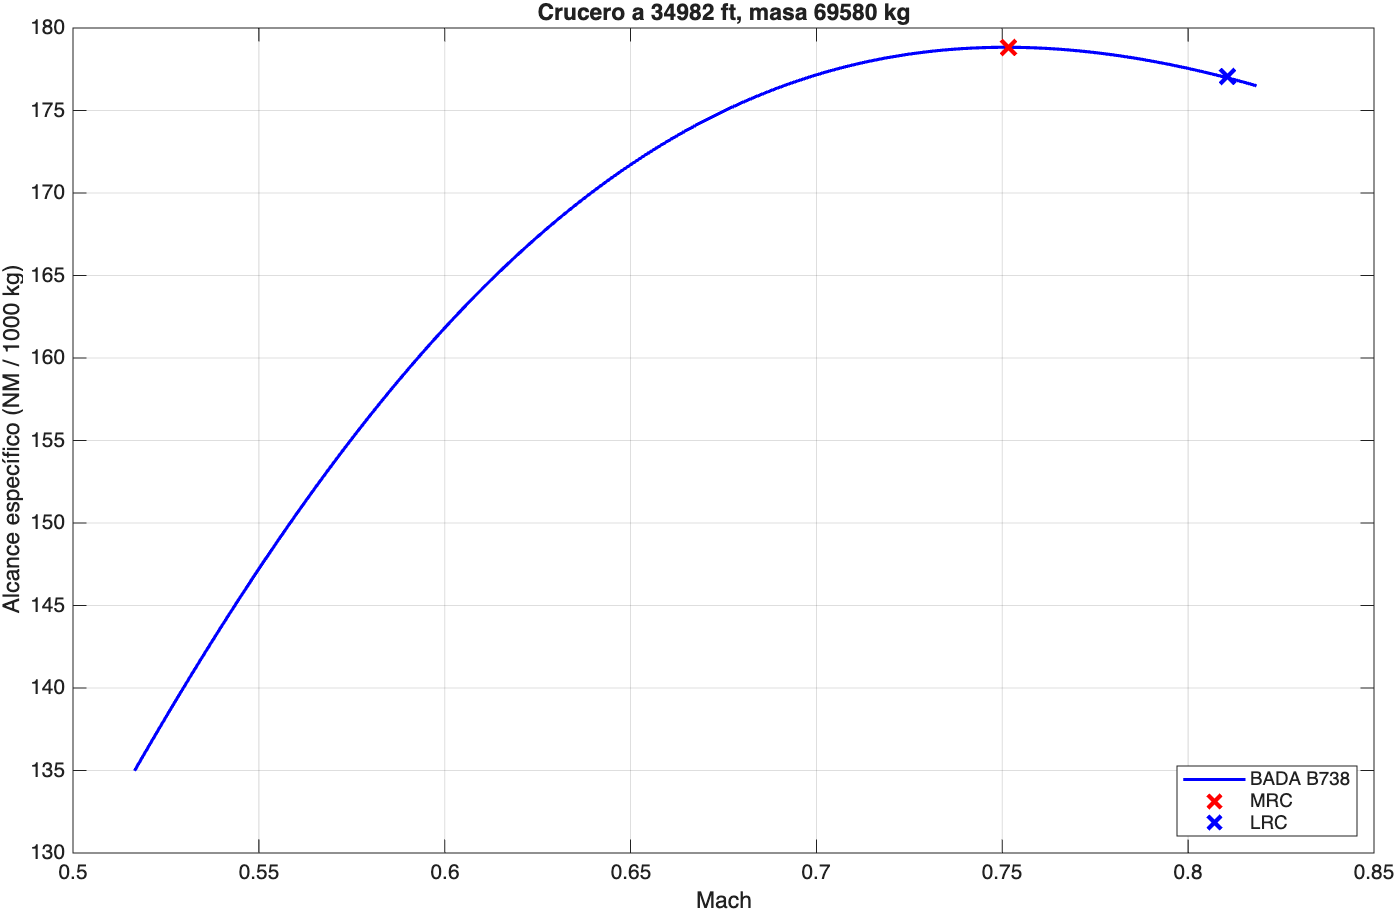
\includegraphics[width=0.72\linewidth]{VERTICAL-MRC.png}
\caption{Alcance específico del B738 (BADA 3.14) en función del Mach a \vHcru~ft y masa media de crucero; MRC (máximo) y LRC (99\,\% del máximo). Fichero \m{VERTICAL-MRC.png}.}
\label{fig:mrc}
\end{figure}

\textbf{Altitudes de cruce.} Con \m{CrossOverAltitude} (\m{kgbx-lib/bada}): ascenso 300~kt/M0,78 $\rightarrow$ \vHcrossClb~ft (igual al valor del ejemplo del enunciado, 29\,314~ft); descenso 290~kt/M0,78 $\rightarrow$ \vHcrossDes~ft; par V$_{MO}$/M$_{MO}$ = 340~kt/0,82 $\rightarrow$ 25\,992~ft (salida por consola de \m{main\_vertical.m}). Por debajo de la altitud de cruce se asciende o desciende a IAS constante y por encima a Mach constante.

\subsection{Modelo de tramo: ecuaciones y tipos}

Cada instante del perfil se evalúa con \m{bada\_leg}, adaptación sin variables globales de \m{BADA\_jet3.m} del curso. Con el modelo de energía total de BADA~3 (manual de usuario, §3.2):
\begin{equation}
(T-D)\,V = m\,g\,\dot h + m\,V\,\dot V \quad\Longrightarrow\quad
\dot h = \frac{(T-D)\,V}{m\,g}\,\mathrm{ESF},\qquad \dot V = \frac{(T-D)}{m}\,(1-\mathrm{ESF}),
\end{equation}
donde $T=T_r\,T_{\max}$ con $T_{\max}$ el empuje máximo de ascenso ISA de BADA (§3.7), $D$ la resistencia de la configuración (§3.6) y ESF el factor de reparto de energía (§3.8), que vale la expresión de IAS constante bajo la altitud de cruce, la de Mach constante encima, o un valor impuesto (0,3 en las aceleraciones en ascenso, §3.8). El consumo (§3.9) es $\dot m = \eta\,T\,C_{fcr}$ con $\eta=C_{f1}(1+V/C_{f2})$, o el mínimo $C_{f3}(1-h/C_{f4})$ cuando $T_r$ es igual o menor que el ralentí. Los dos tipos de tramo son:
\begin{itemize}
\item \textbf{SPD} (velocidad constante, IAS o Mach): se fija $T_r$ (segundo grado de libertad) y resultan $\dot h$ (ROCD) y el FPA. Subtipos: $T_r$ fijo (1,0 en despegue; «red», empuje de ascenso reducido de BADA §3.8, en el resto del ascenso), $T_r$ fijo con ESF impuesto (aceleraciones a altitud casi constante) y $T_r$ = ralentí BADA (descenso idle, $T_r = C_{Tdes}$). Con ESF impuesto la incógnita es también $\dot V$.
\item \textbf{PTH} (ángulo de trayectoria constante): se fija el FPA entre dos puntos y, como segundo grado de libertad, $\mathrm{d}V/\mathrm{d}r$ (diferencia de velocidad entre los dos puntos dividida por su distancia); la incógnita es $T_r = (D + W\sin\gamma + m\dot V)/T_{\max}$, que se informa sin recortar: $T_r$ por debajo del ralentí indica que hacen falta frenos aerodinámicos o un FPA menor (sección~6.2.3 del enunciado). En crucero se usa PTH con FPA = 0 y $\mathrm{d}V/\mathrm{d}r=0$ ($T=D$), o $T_r$ fijo para acelerar/decelerar en nivel.
\end{itemize}
\m{fly\_leg} integra cada tramo por Euler explícito con paso de 1~s (10~s en crucero) hasta la primera condición de fin que se alcance (altitud, distancia de ruta, IAS o Mach), acortando el último paso para cumplirla exactamente, y devuelve la fila de la tabla de tramos y la traza. \m{build\_profile} encadena los tramos.

\subsection{Estructura del perfil}

\paragraph{Ascenso (tramos C).} Sigue el esquema C1--C5 del enunciado con las limitaciones de LEMD AD~2.21 y de la SID:
\begin{itemize}
\item \textbf{C1}: ascenso inicial a V$_2$+20 = \vVIIpIIO~kt con empuje de despegue ($T_r$ = 1, BADA solo modela el empuje máximo de ascenso, que se usa como despegue) y configuración de despegue (flap 5) desde 1\,998~ft hasta 1\,500~ft sobre el aeródromo (\vCItop~ft). Velocidad vertical media \vVSCI~fpm.
\item \textbf{C2}: V$_2$+20 con empuje de ascenso reducido (BADA §3.8, sección~\ref{sec:red}) y flap 1 hasta 3\,000~ft sobre el aeródromo (\vCIItop~ft).
\item \textbf{C3}: por encima de 3\,000~ft AAL se acelera y asciende respetando las IAS máximas de la SID, con el empuje de ascenso reducido y configuración limpia. \m{build\_profile} genera automáticamente los subtramos a partir de los límites de la tabla de la SID: C3.1 aceleración 172 $\rightarrow$ 220~kt (ESF 0,3, límite de MD048; el límite de 210~kt en MD047 ya se cumple porque MD047 se cruza a 172~kt); C3.2 ascenso a 220~kt hasta MD048 (\vMDOIVVIIIh~ft); C3.3 aceleración 220 $\rightarrow$ 240~kt; C3.4 ascenso a 240~kt hasta MD824 (\vMDVIIIIIIVh~ft, por encima de los \sidMDVIIIIIIValt~ft mínimos); C3.5 aceleración 240 $\rightarrow$ 300~kt hasta \vCIIIVh~ft. El límite de 250~kt bajo 10\,000~ft queda cubierto por los de 220 y 240~kt de la carta.
\item \textbf{C4}: ascenso a IAS constante 300~kt hasta la altitud de cruce (\vHcrossClb~ft).
\item \textbf{C5}: ascenso a M0,78 constante hasta \vHcru~ft. \textbf{TOC a \vTOC~NM} del DER (52~NM después de NANDO, en el tramo FENXE--MABUX); ascenso de \vTclb~min y \vFuelClb~kg.
\end{itemize}
Ningún fijo de la SID tiene altitud máxima, por lo que no se insertan tramos planos. En todos los tramos $T_r \le 1$.

\paragraph{Crucero (tramos K).} \textbf{K1}: deceleración en nivel de M0,78 a la MRC (M\vMcru) al ralentí (\vKIlen~NM). \textbf{K2}: crucero a \vHcru~ft y Mach constante, \vCruiseLen~NM, con $T_r$ variando de \vTrKIIini{} a \vTrKIIfin~\% según disminuye la masa. \textbf{K3}: aceleración en nivel de la MRC a M0,78 de descenso con el empuje máximo de crucero (0,95~$T_{\max}$, coeficiente $C_{Tcr}$ de BADA §3.7.2; \vKIIIlen~NM); al ser vuelo nivelado a la altitud de crucero cuenta como crucero, y el TOD es su final. K1--K3 consumen \vFuelCru~kg. \textbf{TOD a \vTOD~NM} del DER (\vTODzukko~NM antes de ZUKKO, \vDesLen~NM del umbral). La posición del TOD se obtiene iterando sobre la masa al final de K2: se integran K3 y el descenso idle desde \vHcru~ft hasta 13\,000~ft para esa masa, su longitud se resta de la distancia de ZUKKO, se vuela K2 hasta ese punto y se repite hasta que la masa converge (20~kg).

\paragraph{Descenso (tramos D).} Se construye con la envolvente inferior de los límites de la transición y la ILS (tabla~\ref{tab:des}, suposición~14) y, a diferencia del enunciado, se calcula hacia delante desde el TOD gracias a la iteración anterior:
\begin{itemize}
\item \textbf{D4}: descenso SPD al ralentí BADA ($T_r$ = C$_{Tdes,high}$ = \vTrIdle~\%): D4.1 a M0,78 hasta la altitud de cruce de descenso (\vHcrossDes~ft; \vVSDIVI~fpm, \vDIVIlen~NM) y D4.2 a 290~kt hasta 13\,000~ft, que se alcanzan exactamente en ZUKKO (\vVSDIVII~fpm, \vDIVIIlen~NM). ZUKKO se cruza a 290~kt: la carta no limita la IAS en ese fijo y el avión está por encima de 10\,000~ft.
\item \textbf{D3}: PTH decelerando de 290 a 250~kt entre ZUKKO (13\,000~ft) y KONFO (10\,000~ft, el mínimo de la ventana 10\,000--11\,000), FPA \vFPADIII°; el $T_r$ requerido (\vTrDIII~\%) queda por debajo del ralentí: se necesitan frenos aerodinámicos o un FPA más suave (p.~ej. KONFO a 11\,000~ft).
\item \textbf{D2}: desde 10\,000~ft hasta el FAP, PTH a 250~kt: D2.1 KONFO $\rightarrow$ ERREZ (9\,000~ft); D2.2 tramo plano a 9\,000~ft ERREZ--IVONA--RAPIV--ALIQA--LEGOH (36,3~NM); D2.3 LEGOH $\rightarrow$ ANOZA (5\,000~ft, FPA \vFPADIIIII°, pendiente 3,6\,\%, muy por debajo del 8\,\% máximo de PANS-OPS para la aproximación inicial); D2.4 ANOZA $\rightarrow$ TOPPU (4\,000~ft; $T_r$ = \vTrDIIIV~\%, de nuevo bajo el ralentí: frenos aerodinámicos); D2.5 TOPPU $\rightarrow$ GALGA (2\,600~ft) decelerando a 185~kt (límite de la carta ILS en el segmento intermedio) con flap 15; D2.6 segmento intermedio plano a 2\,600~ft hasta el FAP decelerando a la velocidad de aproximación final \vVfap~kt (rango 115--160~kt de la categoría C en la figura~21 del enunciado).
\item \textbf{D1}: final por la senda ILS desde el FAP (2\,600~ft) hasta el umbral (183~ft) con FPA \vFPADI° (3° de la carta), flap 30, decelerando hasta V$_{ref}$ = \vVref~kt. V$_{ref}$ calculada con la masa de referencia BADA queda ligeramente por encima del rango V$_{at}$ de la categoría C (121--140~kt); con la masa de aterrizaje real (\vMldg~kg) sería menor.
\end{itemize}
El descenso dura \vTdes~min y consume \vFuelDes~kg. En todos los tramos PTH, $T_r \ge 0$.

\begin{table}[H]\centering\footnotesize
\begin{tabularx}{\linewidth}{llrrlY}\toprule
Fijo & Tramo que termina & $h$ (ft) & IAS (kt) & Config. & Origen del valor\\ \midrule
ZUKKO & D4.2 & 13\,000 & 290 & limpia & máximo de la carta ($-$13\,000); IAS de descenso APF\\
KONFO & D3 & 10\,000 & 250 & limpia & mínimo de la ventana 10\,000--11\,000; 250 kt bajo FL100\\
ERREZ & D2.1 & 9\,000 & 250 & limpia & @9\,000\\
LEGOH & D2.2 & 9\,000 & 250 & limpia & @9\,000 (tramo plano)\\
ANOZA & D2.3 & 5\,000 & 250 & limpia & mínimo +5\,000; máx. 250 kt\\
TOPPU & D2.4 & 4\,000 & 250 & limpia & mínimo +4\,000; máx. 250 kt\\
GALGA & D2.5 & 2\,600 & 185 & flap 15 & IF +2\,600; IAS máx. del segmento intermedio (carta ILS)\\
BG074 & D2.6 & 2\,600 & \vVfap & flap 15 & FAP +2\,600; velocidad de aproximación final cat. C\\
THR21 & D1 & 183 & \vVref & flap 30 & cruce del umbral; V$_{ref}$\\ \bottomrule
\end{tabularx}
\caption{Programa de descenso (tabla \m{D} de \m{main\_vertical.m}): altitud e IAS objetivo en cada fijo y configuración del tramo que termina en él.}
\label{tab:des}
\end{table}

\subsection{Tabla de parámetros por tramo}

Las tablas~\ref{tab:vdef} y~\ref{tab:vnum} reproducen \m{VERTICAL-tramos.xlsx}: para cada uno de los \vNlegs{} tramos (\vNclb{} de ascenso, \vNcru{} de crucero, \vNdes{} de descenso) se da el tipo y subtipo, las variables conocidas e incógnitas, la configuración, y las altitudes, velocidades (IAS, TAS, Mach), velocidad vertical, FPA, empuje relativo, distancia, tiempo y combustible.

\begingroup\scriptsize\setlength{\tabcolsep}{2.8pt}
\begin{longtable}{lll>{\raggedright\arraybackslash}p{2.5cm}ll>{\raggedright\arraybackslash}p{4.3cm}}
\caption{Definición de los tramos del perfil vertical (\texttt{VERTICAL-tramos.xlsx}): tipo (SPD/PTH), segundo grado de libertad (subtipo), variables conocidas e incógnitas y configuración aerodinámica BADA.}\label{tab:vdef}\\
\toprule
Tramo & Tipo & Subtipo & Conocidas & Incógnitas & Config. & Descripción\\
\midrule
\endfirsthead
\multicolumn{7}{l}{\small\itshape (continuación)}\\
\toprule
Tramo & Tipo & Subtipo & Conocidas & Incógnitas & Config. & Descripción\\
\midrule
\endhead
\midrule
\multicolumn{7}{r}{\small\itshape continúa}\\
\endfoot
\bottomrule
\endlastfoot
C1 & SPD & Tr fijo & IAS o Mach, Tr & VS (ROCD), FPA & despegue & \scriptsize Ascenso inicial a V2+20 = 172 kt, empuje de despegue, flaps TO\\
C2 & SPD & Tr fijo & IAS o Mach, Tr & VS (ROCD), FPA & ascenso inicial & \scriptsize V2+20 con empuje de ascenso (reducción por ruido), flaps 1\\
C3.1 & SPD & Tr fijo + ESF & Tr, ESF=0,3 & VS, dV/dt (aceleración) & ascenso & \scriptsize Aceleración 172 $\rightarrow$ 220 kt IAS a empuje de ascenso (ESF 0,3)\\
C3.2 & SPD & Tr fijo & IAS o Mach, Tr & VS (ROCD), FPA & ascenso & \scriptsize Ascenso a IAS constante 220 kt (límite de velocidad hasta MD048)\\
C3.3 & SPD & Tr fijo + ESF & Tr, ESF=0,3 & VS, dV/dt (aceleración) & ascenso & \scriptsize Aceleración 220 $\rightarrow$ 240 kt IAS a empuje de ascenso (ESF 0,3)\\
C3.4 & SPD & Tr fijo & IAS o Mach, Tr & VS (ROCD), FPA & ascenso & \scriptsize Ascenso a IAS constante 240 kt (límite de velocidad hasta MD824)\\
C3.5 & SPD & Tr fijo + ESF & Tr, ESF=0,3 & VS, dV/dt (aceleración) & ascenso & \scriptsize Aceleración 240 $\rightarrow$ 300 kt IAS a empuje de ascenso (ESF 0,3)\\
C4 & SPD & Tr fijo & IAS o Mach, Tr & VS (ROCD), FPA & ascenso & \scriptsize Ascenso a IAS constante 300 kt hasta la altitud de cruce\\
C5 & SPD & Tr fijo & IAS o Mach, Tr & VS (ROCD), FPA & ascenso & \scriptsize Ascenso a Mach constante 0,78 hasta la altitud de crucero\\
K1 & PTH & Tr fijo & FPA, Tr & dV/dt & crucero & \scriptsize Deceleración en nivel M0,78 $\rightarrow$ M0,752 (MRC), ralentí\\
K2 & PTH & dV/dr fijo & FPA, dV/dr (IAS inicial y final) & Tr & crucero & \scriptsize Crucero a 34982 ft y Mach 0,752 constante (MRC) hasta el K3 / TOD\\
K3 & PTH & Tr fijo & FPA, Tr & dV/dt & crucero & \scriptsize Aceleración en nivel M0,752 $\rightarrow$ M0,78 de descenso\\
D4.1 & SPD & Tr ralentí & IAS o Mach, Tr = ralentí (BADA) & VS (ROD), FPA & descenso & \scriptsize Descenso en ralentí a Mach constante 0,78 hasta la altitud de cruce\\
D4.2 & SPD & Tr ralentí & IAS o Mach, Tr = ralentí (BADA) & VS (ROD), FPA & descenso & \scriptsize Descenso en ralentí a IAS constante 290 kt hasta ZUKKO (13000 ft)\\
D3 & PTH & dV/dr fijo & FPA, dV/dr (IAS inicial y final) & Tr & descenso & \scriptsize PTH decelerando 290 $\rightarrow$ 250 kt hasta KONFO (11000 ft, ventana 10000-11000 ft)\\
D2.1 & PTH & dV/dr fijo & FPA, dV/dr (IAS inicial y final) & Tr & descenso & \scriptsize PTH KONFO $\rightarrow$ ERREZ (@9000 ft)\\
D2.2 & PTH & dV/dr fijo & FPA, dV/dr (IAS inicial y final) & Tr & descenso & \scriptsize tramo plano a 9000 ft ERREZ-IVONA-RAPIV-ALIQA-LEGOH\\
D2.3 & PTH & dV/dr fijo & FPA, dV/dr (IAS inicial y final) & Tr & descenso & \scriptsize PTH LEGOH $\rightarrow$ ANOZA (mín. 5000 ft)\\
D2.4 & PTH & dV/dr fijo & FPA, dV/dr (IAS inicial y final) & Tr & descenso & \scriptsize PTH ANOZA $\rightarrow$ TOPPU (mín. 4000 ft)\\
D2.5 & PTH & dV/dr fijo & FPA, dV/dr (IAS inicial y final) & Tr & aproximación & \scriptsize PTH TOPPU $\rightarrow$ GALGA (IF, 2600 ft), IAS $\le$ 185 kt (máximo de la carta ILS en HADAS y DEMOV, aproximaciones iniciales a GALGA), flaps 15\\
D2.6 & PTH & dV/dr fijo & FPA, dV/dr (IAS inicial y final) & Tr & aproximación & \scriptsize segmento intermedio a 2600 ft hasta el FAP, deceleración a Vapp = Vat + 5 kt\\
D1 & PTH & dV/dr fijo & FPA, dV/dr (IAS inicial y final) & Tr & aterrizaje & \scriptsize senda ILS 3 grados hasta el umbral (183 ft), deceleración Vapp $\rightarrow$ Vat, flaps 30\\
\end{longtable}
\endgroup

\begingroup\scriptsize\setlength{\tabcolsep}{2.8pt}
\begin{longtable}{lrrrrrrrrrrrrrr}
\caption{Parámetros de cada tramo (\texttt{VERTICAL-tramos.xlsx}): altitud, IAS y TAS (kt) inicial y final, Mach final, velocidad vertical media, ángulo de trayectoria medio, empuje relativo medio $T_r=T/T_{\max}$, distancia, duración, combustible y masa final. $^{a}$\,Tr requerido < ralentí BADA: frenos aerodinámicos o FPA menor.}\label{tab:vnum}\\
\toprule
Tramo & $h_i$ (ft) & $h_f$ (ft) & IAS$_i$ & IAS$_f$ & TAS$_i$ & TAS$_f$ & $M_f$ & VS (fpm) & FPA (°) & $T_r$ (\%) & $d$ (NM) & $t$ (min) & Comb. (kg) & $m_f$ (kg)\\
\midrule
\endfirsthead
\multicolumn{15}{l}{\small\itshape (continuación)}\\
\toprule
Tramo & $h_i$ (ft) & $h_f$ (ft) & IAS$_i$ & IAS$_f$ & TAS$_i$ & TAS$_f$ & $M_f$ & VS (fpm) & FPA (°) & $T_r$ (\%) & $d$ (NM) & $t$ (min) & Comb. (kg) & $m_f$ (kg)\\
\midrule
\endhead
\midrule
\multicolumn{15}{r}{\small\itshape continúa}\\
\endfoot
\bottomrule
\endlastfoot
C1 & 1\,998 & 3\,498 & 172 & 172 & 177 & 181 & 0,277 & 1\,815 & 5,75 & 100,0 & 2,5 & 0,8 & 94 & 76\,327\\
C2 & 3\,498 & 4\,998 & 172 & 172 & 181 & 185 & 0,285 & 1\,824 & 5,65 & 99,5 & 2,5 & 0,8 & 91 & 76\,236\\
C3.1 & 4\,998 & 5\,420 & 172 & 220 & 185 & 238 & 0,366 & 734 & 1,97 & 99,4 & 2,0 & 0,6 & 64 & 76\,173\\
C3.2 & 5\,420 & 11\,066 & 220 & 220 & 238 & 259 & 0,407 & 2\,445 & 5,58 & 99,4 & 9,5 & 2,3 & 247 & 75\,926\\
C3.3 & 11\,066 & 11\,314 & 220 & 240 & 259 & 283 & 0,445 & 776 & 1,62 & 99,4 & 1,4 & 0,3 & 33 & 75\,893\\
C3.4 & 11\,314 & 20\,790 & 240 & 240 & 283 & 327 & 0,534 & 2\,093 & 3,88 & 99,4 & 23,0 & 4,5 & 419 & 75\,474\\
C3.5 & 20\,790 & 21\,983 & 240 & 300 & 327 & 412 & 0,676 & 604 & 0,92 & 99,5 & 12,2 & 2,0 & 168 & 75\,306\\
C4 & 21\,983 & 29\,315 & 300 & 300 & 412 & 461 & 0,780 & 1\,175 & 1,52 & 99,7 & 45,6 & 6,2 & 484 & 74\,822\\
C5 & 29\,315 & 34\,982 & 300 & 265 & 461 & 450 & 0,780 & 925 & 1,15 & 100,0 & 46,4 & 6,1 & 386 & 74\,436\\
K1 & 34\,982 & 34\,982 & 265 & 254 & 450 & 433 & 0,752 & 0 & 0,00 & 8,7 & 1,8 & 0,2 & 2 & 74\,434\\
K2 & 34\,982 & 34\,982 & 254 & 254 & 433 & 433 & 0,752 & 0 & 0,00 & 77,6 & 1\,728,8 & 239,4 & 9\,669 & 64\,766\\
K3 & 34\,982 & 34\,982 & 254 & 265 & 433 & 450 & 0,780 & 0 & 0,00 & 95,0 & 6,0 & 0,8 & 41 & 64\,725\\
D4.1 & 34\,982 & 30\,889 & 265 & 290 & 450 & 458 & 0,780 & $-$3\,271 & $-$4,08 & 8,7 & 9,4 & 1,3 & 9 & 64\,716\\
D4.2 & 30\,889 & 13\,000 & 290 & 290 & 458 & 349 & 0,553 & $-$2\,214 & $-$3,14 & 8,7 & 53,6 & 8,1 & 77 & 64\,639\\
D3$^{a}$ & 13\,000 & 10\,000 & 290 & 250 & 349 & 289 & 0,452 & $-$1\,367 & $-$2,43 & 4,0 & 11,6 & 2,2 & 26 & 64\,613\\
D2.1 & 10\,000 & 9\,000 & 250 & 250 & 289 & 284 & 0,444 & $-$206 & $-$0,41 & 31,6 & 23,2 & 4,9 & 165 & 64\,449\\
D2.2 & 9\,000 & 9\,000 & 250 & 250 & 284 & 284 & 0,444 & 0 & 0,00 & 35,2 & 36,3 & 7,7 & 293 & 64\,156\\
D2.3 & 9\,000 & 5\,000 & 250 & 250 & 284 & 268 & 0,413 & $-$1\,005 & $-$2,06 & 14,4 & 18,3 & 4,0 & 64 & 64\,091\\
D2.4$^{a}$ & 5\,000 & 4\,000 & 250 & 250 & 268 & 265 & 0,406 & $-$1\,429 & $-$3,04 & 5,2 & 3,1 & 0,7 & 9 & 64\,082\\
D2.5 & 4\,000 & 2\,600 & 250 & 185 & 265 & 192 & 0,293 & $-$811 & $-$2,02 & 14,2 & 6,5 & 1,7 & 29 & 64\,053\\
D2.6 & 2\,600 & 2\,600 & 185 & 150 & 192 & 156 & 0,238 & 0 & 0,00 & 21,4 & 2,1 & 0,7 & 17 & 64\,036\\
D1 & 2\,600 & 183 & 150 & 144 & 156 & 144 & 0,218 & $-$811 & $-$3,06 & 21,7 & 7,4 & 3,0 & 74 & 63\,962\\
\end{longtable}
\endgroup


\subsection{Representación gráfica y comprobación de restricciones}

La figura~\ref{fig:fases} muestra el perfil calculado junto con las altitudes mínima y máxima del estudio horizontal para cada fase, y la figura~\ref{fig:completo} la altitud, las velocidades y el empuje relativo y velocidad vertical a lo largo de toda la ruta. \m{check\_profile} interpola el perfil en los \chkN{} fijos de la ruta y compara altitud e IAS con los límites de las tablas Excel (tabla~\ref{tab:chk}): \textbf{se cumplen los \chkOK{} de \chkN}. En particular, MD824 se cruza a \chkMDVIIIIIIV~ft (mínimo \chkMDVIIIIIIVmin~ft por la pendiente del 5,5\,\%), con IAS 240~kt; NANDO a \chkNANDO~ft; ZUKKO a \chkZukkoH~ft y \chkZukkoIAS~kt; KONFO, ERREZ--LEGOH, ANOZA, TOPPU, GALGA y BG074 exactamente a sus altitudes objetivo. Los límites de altitud de las aerovías no se han podido comprobar (sección~\ref{sec:enr-pendiente}); el crucero a \vHcru~ft deberá contrastarse con ellos cuando se completen.

\begin{figure}[!htbp]\centering
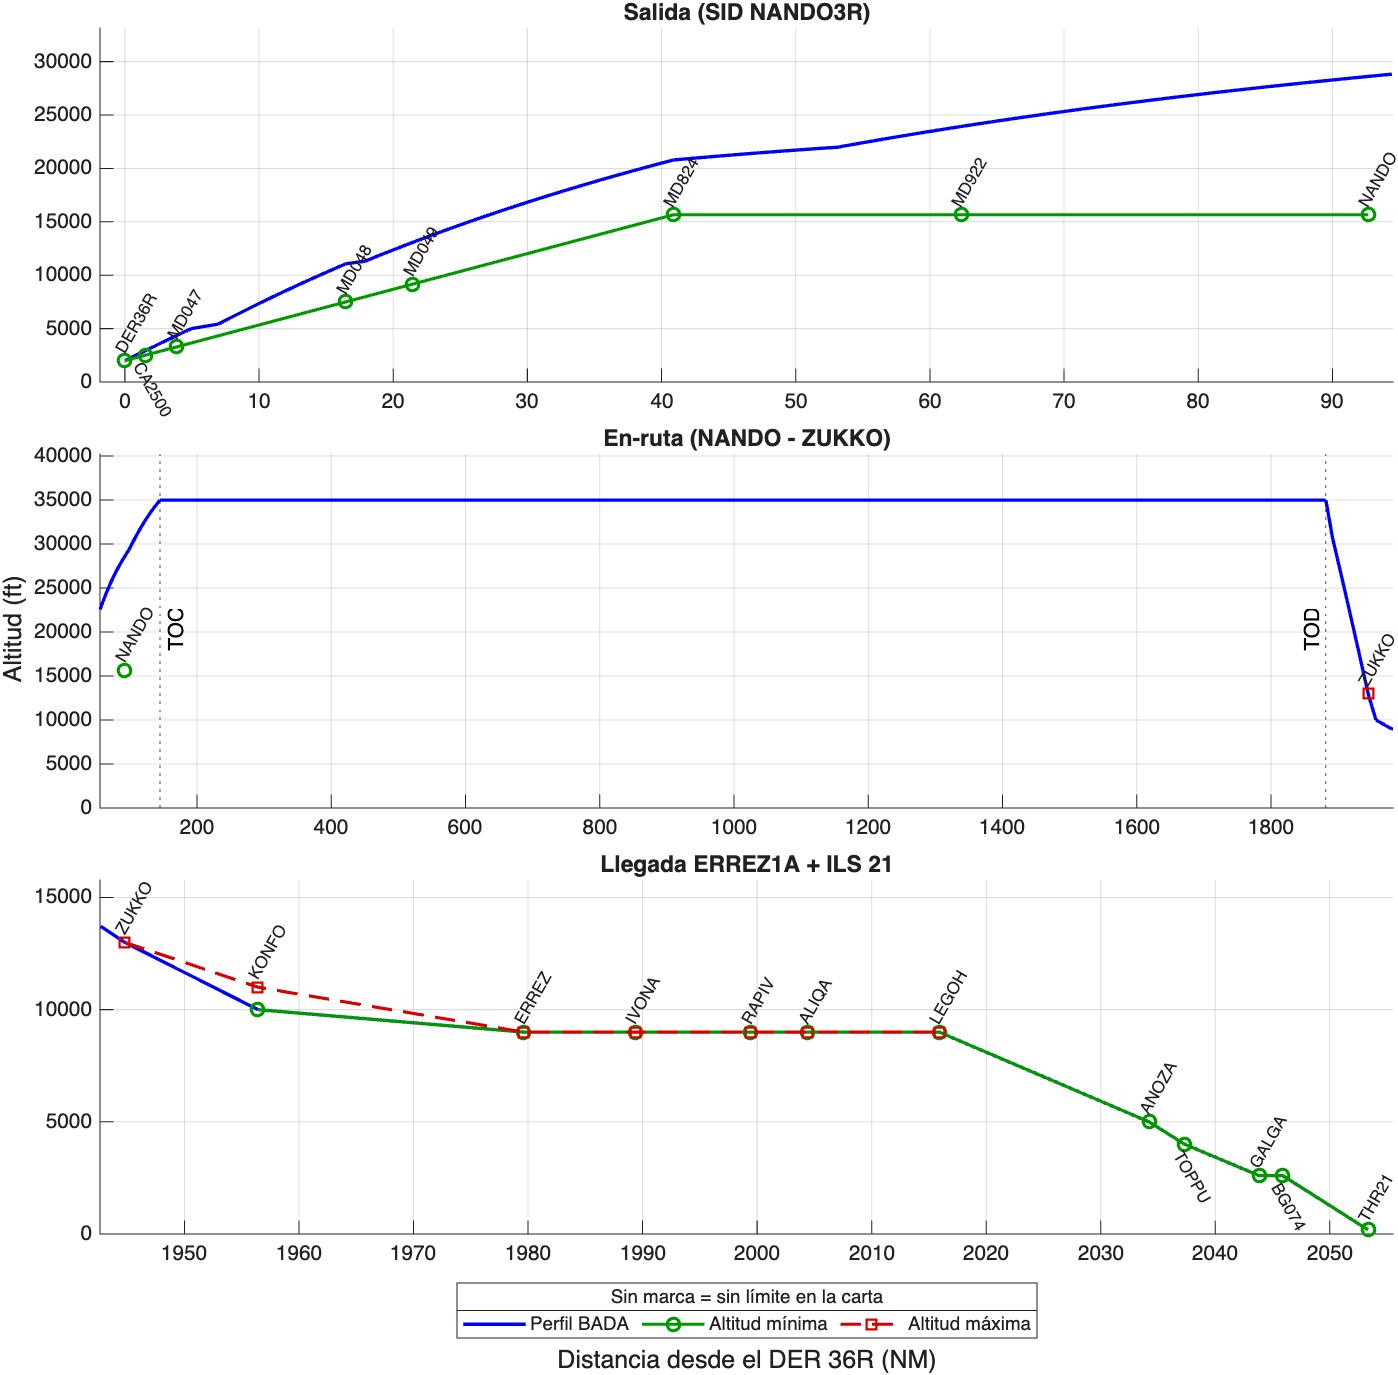
\includegraphics[width=\linewidth]{VERTICAL-perfil-fases.png}
\caption{Perfil vertical BADA (azul) frente a las altitudes mínima (verde) y máxima (rojo) de cada fase: salida, en-ruta y llegada + ILS 21. Las líneas punteadas verticales son el TOC y el TOD. Los límites que la carta no da (mínimo 0~ft, máximo 40\,000~ft) no se dibujan; por eso ZUKKO solo lleva su máxima. Fichero \m{VERTICAL-perfil-fases.png}.}
\label{fig:fases}
\end{figure}

\begin{figure}[!htbp]\centering
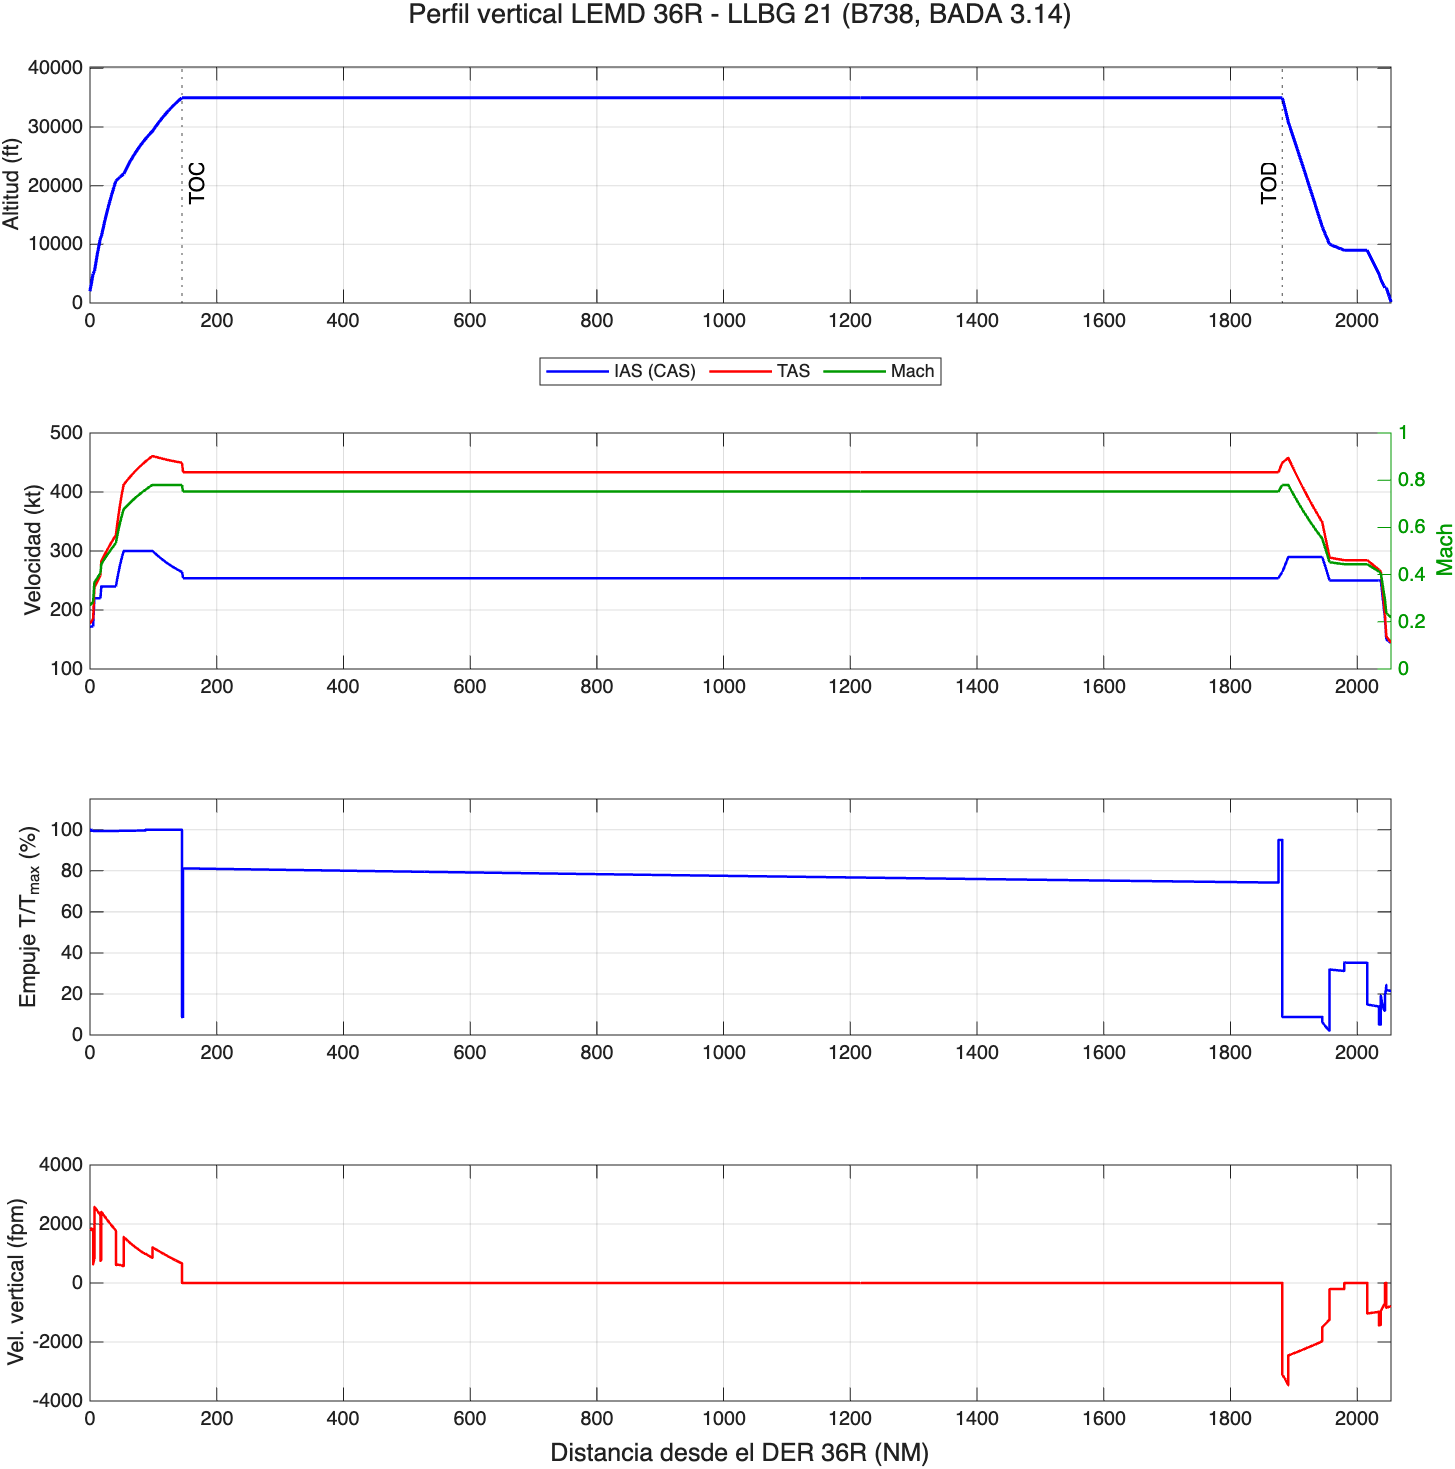
\includegraphics[width=\linewidth]{VERTICAL-perfil-completo.png}
\caption{Ruta completa, de arriba abajo: altitud (con TOC y TOD), IAS/TAS/Mach, empuje relativo y velocidad vertical frente a la distancia desde el DER 36R. Los saltos estrechos del empuje junto al TOC y al TOD son los tramos cortos K1 (ajuste de Mach en ralentí) y K3 (cambio de Mach antes del TOD) de la tabla~\ref{tab:vnum}. Fichero \m{VERTICAL-perfil-completo.png}.}
\label{fig:completo}
\end{figure}

\begingroup\scriptsize\setlength{\tabcolsep}{2.8pt}
\begin{longtable}{lrrrrrrc}
\caption{Comprobación del perfil vertical en los fijos de la ruta (\texttt{VERTICAL-comprobacion.xlsx}): altitud e IAS interpoladas del perfil frente a los límites del estudio horizontal (-- = sin límite; los de las aerovías están pendientes de verificar).}\label{tab:chk}\\
\toprule
Fijo & $D$ (NM) & $h$ perfil (ft) & IAS perfil (kt) & Alt mín (ft) & Alt máx (ft) & IAS máx (kt) & Cumple\\
\midrule
\endfirsthead
\multicolumn{8}{l}{\small\itshape (continuación)}\\
\toprule
Fijo & $D$ (NM) & $h$ perfil (ft) & IAS perfil (kt) & Alt mín (ft) & Alt máx (ft) & IAS máx (kt) & Cumple\\
\midrule
\endhead
\midrule
\multicolumn{8}{r}{\small\itshape continúa}\\
\endfoot
\bottomrule
\endlastfoot
DER36R & 0,0 & 1\,998 & 172 & 1\,998 & 40\,000 & 250 & sí\\
CA2500 & 1,5 & 2\,926 & 172 & 2\,500 & 40\,000 & 250 & sí\\
MD047 & 3,9 & 4\,359 & 172 & 3\,291 & 40\,000 & 210 & sí\\
MD048 & 16,5 & 11\,066 & 220 & 7\,501 & 40\,000 & 220 & sí\\
MD049 & 21,4 & 13\,071 & 240 & 9\,165 & 40\,000 & 250 & sí\\
MD824 & 40,9 & 20\,790 & 240 & 15\,660 & 40\,000 & 240 & sí\\
MD922 & 62,3 & 23\,928 & 300 & 15\,660 & 40\,000 & 350 & sí\\
NANDO & 92,7 & 28\,612 & 300 & 15\,660 & 40\,000 & 350 & sí\\
FENXE & 125,6 & 32\,990 & 277 & -- & -- & -- & sí\\
MABUX & 146,8 & 34\,982 & 255 & -- & -- & -- & sí\\
RETBA & 159,7 & 34\,982 & 254 & -- & -- & -- & sí\\
MOPIR & 163,4 & 34\,982 & 254 & -- & -- & -- & sí\\
LASPO & 179,1 & 34\,982 & 254 & -- & -- & -- & sí\\
ORVUS & 224,6 & 34\,982 & 254 & -- & -- & -- & sí\\
GODOX & 270,1 & 34\,982 & 254 & -- & -- & -- & sí\\
EDULI & 316,9 & 34\,982 & 254 & -- & -- & -- & sí\\
PTC & 355,8 & 34\,982 & 254 & -- & -- & -- & sí\\
SOTAX & 421,8 & 34\,982 & 254 & -- & -- & -- & sí\\
RISEP & 437,0 & 34\,982 & 254 & -- & -- & -- & sí\\
ETOIL & 537,5 & 34\,982 & 254 & -- & -- & -- & sí\\
XATOS & 576,2 & 34\,982 & 254 & -- & -- & -- & sí\\
IBREP & 581,3 & 34\,982 & 254 & -- & -- & -- & sí\\
ADEXI & 851,8 & 34\,982 & 254 & -- & -- & -- & sí\\
OLLEK & 942,3 & 34\,982 & 254 & -- & -- & -- & sí\\
NEVIK & 1\,310,5 & 34\,982 & 254 & -- & -- & -- & sí\\
PLH & 1\,395,1 & 34\,982 & 254 & -- & -- & -- & sí\\
TIPUS & 1\,442,1 & 34\,982 & 254 & -- & -- & -- & sí\\
OTREX & 1\,457,0 & 34\,982 & 254 & -- & -- & -- & sí\\
AMAXI & 1\,498,6 & 34\,982 & 254 & -- & -- & -- & sí\\
SIT & 1\,518,6 & 34\,982 & 254 & -- & -- & -- & sí\\
VANZA & 1\,707,2 & 34\,982 & 254 & -- & -- & -- & sí\\
PIKOG & 1\,922,0 & 20\,719 & 290 & -- & -- & -- & sí\\
ZUKKO & 1\,944,8 & 13\,000 & 290 & 0 & 13\,000 & 350 & sí\\
KONFO & 1\,956,4 & 10\,000 & 250 & 10\,000 & 11\,000 & 350 & sí\\
ERREZ & 1\,979,6 & 9\,000 & 250 & 9\,000 & 9\,000 & 250 & sí\\
IVONA & 1\,989,4 & 9\,000 & 250 & 9\,000 & 9\,000 & 250 & sí\\
RAPIV & 1\,999,4 & 9\,000 & 250 & 9\,000 & 9\,000 & 250 & sí\\
ALIQA & 2\,004,4 & 9\,000 & 250 & 9\,000 & 9\,000 & 250 & sí\\
LEGOH & 2\,015,9 & 9\,000 & 250 & 9\,000 & 9\,000 & 250 & sí\\
ANOZA & 2\,034,2 & 5\,000 & 250 & 5\,000 & 40\,000 & 250 & sí\\
TOPPU & 2\,037,3 & 4\,000 & 250 & 4\,000 & 40\,000 & 250 & sí\\
GALGA & 2\,043,8 & 2\,600 & 185 & 2\,600 & 40\,000 & 250 & sí\\
BG074 & 2\,045,9 & 2\,600 & 150 & 2\,600 & 40\,000 & 250 & sí\\
THR21 & 2\,053,3 & 183 & 144 & 183 & 40\,000 & 250 & sí\\
\end{longtable}
\endgroup


\subsection{Combustible y tiempo; comparación de velocidades y altitudes de crucero}

Para el perfil propuesto (\vHcru~ft, MRC) el combustible DER--umbral es \vFuelClb{} (ascenso) + \vFuelCru{} (crucero) + \vFuelDes{} (descenso) = \textbf{\vFuelTot~kg}, el tiempo \vTime{} (\vTimeh~h) y la masa de aterrizaje \vMldg~kg. El reparto sigue la altitud: todo tramo nivelado a la altitud de crucero (K1--K3, incluido el cambio de Mach previo al TOD) es crucero, y el descenso empieza en el TOD. La tabla~\ref{tab:consumo} (\m{VERTICAL-consumo.xlsx}) repite el cálculo completo para dos altitudes (\cHI{} y \cHII~ft) y dos velocidades (MRC y LRC de cada altitud, misma masa de referencia):

\begin{table}[htbp]
\centering
\scriptsize\setlength{\tabcolsep}{3.5pt}
\caption{Consumo y tiempo de vuelo (DER 36R a THR 21) para dos altitudes y dos velocidades de crucero (\texttt{VERTICAL-consumo.xlsx}), misma masa de referencia de crucero.}\label{tab:consumo}
\begin{tabular}{rlrrrrrrrrr}
\toprule
$h$ (ft) & Vel. & Mach & TOC (NM) & TOD (NM) & Crucero (NM) & Asc. (kg) & Cru. (kg) & Des. (kg) & Total (kg) & $t$ (h)\\
\midrule
34\,982 & MRC & 0,752 & 145,1 & 1\,881,8 & 1\,736,7 & 1\,985,2 & 9\,710,8 & 747,4 & 12\,443,3 & 4,97\\
34\,982 & LRC & 0,810 & 145,1 & 1\,881,8 & 1\,736,7 & 1\,985,2 & 9\,810,6 & 746,9 & 12\,542,7 & 4,68\\
31\,000 & MRC & 0,687 & 110,1 & 1\,891,2 & 1\,781,1 & 1\,701,4 & 10\,504,2 & 736,1 & 12\,941,7 & 5,28\\
31\,000 & LRC & 0,742 & 110,1 & 1\,891,3 & 1\,781,2 & 1\,701,4 & 10\,614,4 & 735,6 & 13\,051,3 & 4,96\\
\bottomrule
\end{tabular}
\end{table}


\begin{itemize}
\item A \cHI~ft, la LRC (M\cMachLRCI) gasta \cDiffLRCI~kg más que la MRC (el 1\,\% de alcance específico que la define, compensado en parte porque el paso a M0,78 antes del TOD es entonces una deceleración al ralentí y no una aceleración) y ahorra \cDiffTLRCI~min.
\item Bajar a \cHII~ft cuesta \cDiffH~kg más con MRC: el consumo de crucero sube y, además, la MRC de BADA a esa altitud (M\cMachMRCII) es mucho más lenta, por lo que el vuelo dura \cTMRCII~h. A \cHII~ft el TOC se adelanta a \cTOCII~NM.
\item El resultado confirma la regla de la sección~6.3.2 del enunciado: para esta ruta la altitud más alta y la MRC son la combinación de mínimo consumo; la LRC es la elección razonable si se valora el tiempo.
\end{itemize}

\subsection{Empuje de ascenso reducido (BADA 3.8)}\label{sec:red}

En lugar de suponer un valor de palanca para el «empuje de ascenso» tras la reducción de ruido, se aplica el modelo de potencia de ascenso reducida del manual BADA~3 (§3.8): el exceso de potencia se multiplica por
\begin{equation}
C_{pow,red} = 1 - C_{red}\,\frac{m_{\max}-m}{m_{\max}-m_{\min}},\qquad C_{red} = 0{,}15 \text{ (reactores)},
\end{equation}
solo por debajo de $0{,}8\,h_{\max}$ (27\,986~ft). \m{bada\_leg} (modo \m{known = 'red'}) obtiene el empuje que da ese exceso: $T = D + C_{pow,red}(T_{\max}-D)$. Con la masa de este vuelo (\sbTOW~kg, próxima a la máxima) $C_{pow,red}\approx0{,}992$ y el $T_r$ resultante en C2--C4 está entre 99,4 y 99,7\,\% (tabla~\ref{tab:vnum}); por encima de 27\,986~ft (final de C4 y C5) es el 100\,\%. La reducción es pequeña porque el B738 despega casi a masa máxima.

% ============================================================ 7
\section{Conclusiones}

\paragraph{Procedimientos trabajados y disponibilidad.} La ruta LEMD~36R $\rightarrow$ LLBG~21 permite ejercitar todos los tipos de procedimiento del enunciado con cartas oficiales vigentes: una SID RNAV~1 con tramo CA inicial, tramos CF/TF, pendiente mínima operacional del 5,5\,\% y limitaciones de velocidad escalonadas (NANDO3R, AIP ENAIRE); un tramo en-ruta de \enrDist~NM que combina aerovías convencionales (T257, UL144, UM978, L609) con espacios de ruta libre; una transición RNAV~1 a la aproximación con carta propia, esperas y un segmento a altitud fija (ERREZ1A, eAIP Israel); una aproximación de precisión ILS CAT~I y una de no precisión RNP~APCH con tramo RF, con frustrada común que impone un gradiente del 4,5\,\%. LLBG publica para la pista 21 las aproximaciones ILS, LOC y RNP~Y (además de RNP para otras pistas) y la transición desde ZUKKO/KONFO/ERREZ; LEMD publica para la 36R las SID BARDI, CCS, NANDO y PINAR en la carta SID~7. La distancia total es \vTotalD~NM del DER al umbral (SID \sidDist, en-ruta \enrDist, transición \arrDist, ILS \arrToppuRest~NM); por la RNP~Y la aproximación sería \rnpDist~NM.

\paragraph{Resultados principales.} Sin viento, el en-ruta se vuela en \enrTnoW{} a 450~kt; con el viento previsto (de cola en casi toda la ruta) y el criterio literal del enunciado, en \enrTW{}, y en \enrTWg{} si el tiempo se calcula con la GS. Para el perfil vertical con BADA, el B738 alcanza el TOC a \vTOC~NM, cruza a \vHcru~ft y M\vMcru{} (MRC) durante \vCruiseLen~NM, inicia el descenso en el TOD a \vTOD~NM y consume \vFuelTot~kg en \vTime, cumpliendo los \chkN{} límites de altitud y velocidad identificados en el estudio horizontal.

\paragraph{Comparación con SimBrief.} El plan LIDO estima \sbBurn~kg de combustible de etapa y \sbTime{} de vuelo con una masa de aterrizaje de \sbLDW~kg; el modelo BADA da \vFuelTot~kg (+\sbDiffFuel~kg, +\sbDiffFuelPct~\%) y \vMldg~kg de masa de aterrizaje. La coherencia es buena teniendo en cuenta las diferencias de planteamiento: SimBrief vuela con índice de coste \sbCI{} a M\sbMach{} (\sbTAS~kt TAS) con escalones de nivel (\sbSteps) y viento de cola medio de 28~kt, en \sbDist~NM con la SID/STAR de su base de datos; el perfil BADA vuela sin viento, a MRC (más lenta: de ahí los 34~min más de duración) y a un nivel único, sobre \vTotalD~NM con los procedimientos vigentes. La MRC de BADA~3 es además baja por la ausencia de resistencia de compresibilidad en su polar.

\paragraph{Lecciones.} (1) Los calculadores de ruta no sustituyen al AIP: el plan SimBrief usaba un ciclo AIRAC de 2025 y sus SID y STAR no existen en las cartas actuales, y el enlace entre transición y aproximación (TOPPU $\rightarrow$ GALGA o GINTU) solo se entiende leyendo la carta. (2) La precisión geométrica depende de leer bien las tablas de codificación: las distancias calculadas reproducen las de las cartas con error inferior a 0,1~NM, lo que valida las coordenadas; el arco RF se aproxima con puntos cada 10°. (3) El criterio de tiempo con viento del enunciado (rumbo constante, $t=d/\mathrm{TAS}$) produce un vuelo que se separa de la ruta hasta \enrDevMax~NM y una duración distinta de la que daría $t=d/\mathrm{GS}$; conviene presentar ambos. (4) En el perfil vertical, la separación entre tramos SPD (ascenso y descenso idle, con $T_r$ fijo y ROCD resultante) y PTH (descenso guiado por altitudes de carta, con $T_r$ resultante) explica dónde se necesitan frenos aerodinámicos: en esta ruta, en ZUKKO $\rightarrow$ KONFO y ANOZA $\rightarrow$ TOPPU. (5) La reducción de potencia de ascenso de BADA depende de la masa y es casi nula cerca de la MTOW. (6) El diseño modular (cuatro programas principales y una biblioteca de funciones con las tablas de los procedimientos como únicos datos) permite cambiar de ruta sin tocar las funciones (apéndice~\ref{ap:otra-ruta}).

\paragraph{Limitaciones y trabajo pendiente.} Las más importantes son las que se marcan como pendientes en el texto: los fijos, aerovías y descripciones de ruta libre fuera de España y Francia, y los límites de altitud de todas las aerovías, no se han verificado contra sus AIP, y las cartas deben recomprobarse con el AIRAC 002/2026 (26-nov-2026). El modelo tiene además simplificaciones de alcance: no se integran las esperas ni la frustrada en el perfil vertical; la frustrada se representa solo como THR21 $\rightarrow$ GEMDA; la RNP~Y no tiene perfil vertical; las velocidades de ascenso/descenso proceden del APF de BADA y no de la base de prestaciones de Eurocontrol; V$_2$ y V$_{ref}$ se estiman a partir de las V$_{stall}$ de BADA; el viento de cada tramo es el del fijo inicial y solo se aplica al en-ruta; y los KML llevan altitud 0 (perfil horizontal), aunque el campo \m{alt} está preparado para volcar el perfil vertical.

% ============================================================ APENDICES
\appendix
\clearpage
\section{Explicación de las funciones MATLAB}\label{ap:funciones}

El código está en \m{matlab/}: cuatro programas principales (\m{main\_enroute.m}, \m{main\_sid.m}, \m{main\_star\_app.m}, \m{main\_vertical.m}), que solo contienen los datos de la ruta y las llamadas, y la biblioteca \m{matlab/lib/} con las funciones que se describen a continuación en el formato del apéndice~B del enunciado. Se ejecutan desde \m{matlab/} con \m{matlab -batch main\_xxx}; las salidas van a \m{matlab/out/}. Se apoyan en las bibliotecas del curso: \m{kgbx-lib/geo} (\m{orto\_distazi}, \m{orto\_reckon}), \m{kgbx-lib/kml} (\m{create\_wp}, \m{create\_attr}, \m{kmlwrite\_polyline}), \m{kgbx-lib/bada} (\m{LoadAircraftBADA}, \m{CrossOverAltitude}, \m{cas2tas}, \m{tas2cas}, \m{getAtmosphericData}), \m{matlab\_utilities} (\m{maxCruiseAlt}) y \m{simbrief-flightplan-example} (\m{fill\_wp}). La función \m{xml2struct} del curso no funciona en MATLAB R2026b (usa \m{toCharArray}, eliminada); se incluye una copia corregida en \m{matlab/lib/xml2struct\_r2026/} sin modificar la original.

\subsection*{A.1 Programas principales}

\begin{description}[style=nextline]
\item[\m{main\_enroute.m}] Importa NANDO--ZUKKO del plan LIDO (\m{read\_enroute\_wp}), añade los campos \m{alt\_min}/\m{alt\_max} (límites de aerovía, pendientes), calcula distancias (\m{route\_distances}), tiempos sin y con viento (\m{route\_time\_nowind}, \m{route\_time\_wind}) y escribe \m{enroute-sinviento.kml/.xlsx}, \m{enroute-conviento.kml/.xlsx} (este último con las posiciones reales); \m{plot\_enroute\_map} dibuja el mapa de la figura~\ref{fig:mapa}.
\item[\m{main\_sid.m}] Contiene la tabla \m{P} de la SID NANDO3R (nombre, coordenadas de la carta, altitud mínima, IAS máxima, descripción), la elevación y la pendiente mínima; calcula el punto CA2500, las distancias y las restricciones (\m{apply\_restrictions}) y escribe \m{SID-NANDO3R.kml/.xlsx} y la gráfica de límites.
\item[\m{main\_star\_app.m}] Contiene las tablas \m{P} (ERREZ1A + ILS 21), \m{M} (frustrada) y \m{PR} (RNP Y 21, con los puntos del arco RF de \m{add\_arc\_points}); calcula distancias restantes (\m{to\_remaining\_dist}) y límites (\m{apply\_chart\_limits}) y escribe los cuatro KML, las cuatro tablas y las tres gráficas.
\item[\m{main\_vertical.m}] Carga el B738 de BADA, lee las tablas de las fases (\m{load\_phase\_table}), define los parámetros \m{P} (TOW de SimBrief, V$_2$, alturas de reducción de empuje y aceleración, velocidades APF, altitud de crucero y de cruce) y el programa de descenso \m{D}; calcula la MRC (\m{cruise\_speeds}) en dos pasadas, construye el perfil (\m{build\_profile}), lo comprueba (\m{check\_profile}), escribe \m{VERTICAL-tramos.xlsx}, \m{VERTICAL-comprobacion.xlsx}, \m{VERTICAL-consumo.xlsx} y las figuras, y repite el perfil para 2 altitudes $\times$ 2 velocidades.
\end{description}

\subsection*{A.2 Funciones del estudio horizontal}

\funcion{read\_enroute\_wp(xmlfile, firstFix, lastFix)}
{\m{xmlfile} = string, ruta del XML del plan LIDO de SimBrief; \m{firstFix}, \m{lastFix} = string, identificadores del primer y último fijo a importar (p.~ej. 'NANDO', 'ZUKKO')}
{\m{wp} = vector de struct tipo waypoint (campos de \m{create\_wp}: name, lat, lon, alt, desc, tas, head, gs, track, vr, wind, wdir, dist, time) con nombre, descripción, coordenadas y previsión de viento rellenos}
{Convierte el XML con \m{xml2struct}, localiza los índices de los dos fijos en \m{OFP.navlog.fix}, y llama a \m{fill\_wp} para cada fijo entre ambos saltando los pseudofijos TOC y TOD de SimBrief.}

\funcion{route\_distances(wp)}
{\m{wp} = vector de struct con lat y lon (grados)}
{\m{wp} con \m{track} (derrota inicial del tramo que llega al fijo, grados), \m{dist} (distancia de ese tramo, m) y \m{Total\_dist} (acumulada, m); el primer fijo lleva ceros}
{Para cada pareja de fijos consecutivos calcula distancia y acimut ortodrómicos con \m{orto\_distazi} y acumula la distancia. Convención de la figura~2 del enunciado.}

\funcion{route\_time\_nowind(wp, tas)}
{\m{wp} = vector de struct con \m{dist} (m); \m{tas} = double, TAS de crucero (kt)}
{\m{wp} con \m{tas}, \m{gs} y \m{GS} (= TAS), \m{head} (= derrota) y \m{time} (s, acumulado desde el primer fijo)}
{Caso sin viento: la GS es la TAS y el tiempo de cada tramo es \m{dist}/TAS.}

\funcion{computeWT(lat1, lon1, lat2, lon2, windSpeed, windDir, tas)}
{\m{lat1, lon1} = double, punto inicial (grados); \m{lat2, lon2} = double, destino deseado (grados); \m{windSpeed} = double, intensidad del viento (kt); \m{windDir} = double, dirección de procedencia del viento (grados, como en LIDO); \m{tas} = double opcional, TAS (kt), 450 por defecto}
{\m{GS} = double, módulo de la velocidad sobre el suelo (kt); \m{track} = double, derrota real (grados); \m{latD, lonD} = double, coordenadas del destino efectivo}
{Resuelve el tercer caso del triángulo de velocidades (sección~3.2 del enunciado): rumbo = acimut inicial hacia el destino (\m{orto\_distazi}); vector GS = vector TAS + vector viento (dirección del viento + 180°); tiempo = distancia/TAS; destino efectivo = \m{orto\_reckon} desde el origen a GS$\cdot t$ sobre la derrota real.}

\funcion{route\_time\_wind(wp, tas)}
{\m{wp} = vector de struct con lat, lon, wind, wdir; \m{tas} = double (kt)}
{\m{wv} = copia de \m{wp} con \m{tas}, \m{head} (rumbo = derrota deseada desde la posición real), \m{gs}/\m{GS}, \m{track} (derrota real), \m{dist} (m, desde la posición real), \m{Total\_dist}, \m{time} (s, criterio $d$/TAS), \m{time\_gs} (s, criterio $d$/GS), \m{lat\_real}, \m{lon\_real} (posición alcanzada) y \m{dev\_m} (distancia entre la posición real y el fijo, m)}
{Llama a \m{computeWT} tramo a tramo; cada tramo parte de la posición real alcanzada en el anterior y usa como viento la previsión del fijo planificado en que empieza. Acumula los dos tiempos.}

\funcion{export\_route\_table(file, wp)}
{\m{file} = string, nombre del fichero sin extensión; \m{wp} = vector de struct con los campos de la tabla}
{Fichero \m{file.xlsx} con las columnas de la figura~2 del enunciado: número, nombre, latitud, longitud, altitud mínima y máxima, derrota, distancia (NM), distancia total (NM), dirección e intensidad del viento, GS y tiempo total (s)}
{Monta una celda con cabecera y una fila por fijo (distancias convertidas de m a NM) y la escribe con \m{writecell}. Sustituye a \m{myxlswrite\_ENR} del curso.}

\funcion{dms2deg(s)}
{\m{s} = char, coordenada en formato AIP: 'ddmmss.sN' o 'dddmmss.sW' (p.~ej. '403537.1N', '0033217.6W')}
{\m{deg} = double, grados decimales (negativos para S y W)}
{Separa grados, minutos y segundos contando desde el punto decimal (o el final) y aplica el signo según el hemisferio. Admite segundos con o sin decimales.}

\funcion{build\_procedure(P)}
{\m{P} = cell array, una fila por punto: \{nombre, 'lat', 'lon', altMinCarta, iasMaxCarta, descripción [, altMaxCarta]\}; las coordenadas pueden ser cadenas AIP o números en grados decimales; NaN cuando la carta no da límite}
{\m{wp} = vector de struct tipo waypoint con name, lat, lon, desc, \m{alt\_chart}, \m{ias\_chart}, \m{alt\_max\_chart} y los campos \m{alt\_min}, \m{alt\_max}, \m{ias\_min}, \m{ias\_max}, \m{slope}, \m{Total\_dist}, \m{GS} inicializados}
{Crea cada waypoint con \m{create\_wp}, convierte las coordenadas con \m{dms2deg} si son cadenas y copia los límites de la carta. Es la única forma de introducir un procedimiento: la carta se transcribe a la tabla \m{P} y nada más.}

\funcion{add\_arc\_points(cLat, cLon, r\_NM, brg1, brg2, clockwise, stepDeg, prefix, altMin, iasMax)}
{\m{cLat, cLon} = double, centro del arco (grados); \m{r\_NM} = double, radio (NM); \m{brg1, brg2} = double, marcaciones del centro al inicio y al final del arco (grados); \m{clockwise} = logical, viraje a la derecha; \m{stepDeg} = double, paso angular (grados); \m{prefix} = string, prefijo de los nombres; \m{altMin}, \m{iasMax} = double, límites que heredan los puntos}
{\m{R} = cell array de filas en el formato de \m{build\_procedure} con los puntos intermedios del arco (vacío si el arco es más corto que el paso)}
{Calcula el ángulo barrido en el sentido indicado y genera con \m{orto\_reckon} un punto a distancia \m{r\_NM} del centro cada \m{stepDeg} grados, excluidos los extremos. Sirve para tramos RF (y arcos DME).}

\funcion{apply\_restrictions(wp, elev\_ft, grad, lastGradFix, altMaxDefault, iasMaxDefault)}
{\m{wp} = vector de struct con \m{Total\_dist} (m), \m{alt\_chart}, \m{alt\_max\_chart}, \m{ias\_chart}; \m{elev\_ft} = double, elevación inicial (ft); \m{grad} = double, pendiente mínima (fracción, 0,055); \m{lastGradFix} = string, último fijo al que se aplica la pendiente; \m{altMaxDefault} = double, altitud «sin límite» (ft); \m{iasMaxDefault} = double, IAS «sin límite» (kt)}
{\m{wp} con \m{alt\_min} (máximo entre la carta y la altitud de la pendiente; tras \m{lastGradFix} se mantiene la anterior), \m{alt\_max} (carta o valor por defecto), \m{ias\_min} (0), \m{ias\_max} (carta; si no, 250 kt bajo 10\,000 ft; si no, valor por defecto) y \m{slope} (pendiente del tramo entre altitudes mínimas, \%)}
{Función de restricciones de la SID (sección~4 del enunciado). La pendiente se aplica a la distancia acumulada desde el primer punto.}

\funcion{apply\_chart\_limits(wp, altMaxDefault, iasMaxDefault)}
{\m{wp} = vector de struct con \m{alt\_chart}, \m{alt\_max\_chart}, \m{ias\_chart}; \m{altMaxDefault}, \m{iasMaxDefault} = double, valores «sin límite»}
{\m{wp} con \m{alt\_min} (carta o 0), \m{alt\_max} (carta o valor por defecto), \m{ias\_min} (0) e \m{ias\_max} (carta; 250 kt si el fijo está por debajo de 10\,000 ft; valor por defecto en caso contrario, incluido un fijo sin altitud mínima cuya máxima es $\ge$ 10\,000 ft, como ZUKKO)}
{Variante de \m{apply\_restrictions} para llegada y aproximación, sin pendiente mínima. Un límite «@» se introduce como mínimo = máximo.}

\funcion{to\_remaining\_dist(wp)}
{\m{wp} = vector de struct con \m{Total\_dist} acumulada (m)}
{\m{wp} con \m{Total\_dist} convertida en distancia restante hasta el último fijo (umbral)}
{Resta cada acumulada del total. Se usa en llegada y aproximación (sección~5 del enunciado).}

\funcion{export\_proc\_table(file, wp, distLabel)}
{\m{file} = string, nombre sin extensión; \m{wp} = vector de struct; \m{distLabel} = string, título de la columna de distancia total ('Distancia total (NM)', 'Distancia restante a THR21 (NM)' o, en la frustrada, 'Distancia total desde THR21 (NM)')}
{Fichero \m{file.xlsx} con las columnas de la figura~14 del enunciado (número, nombre, latitud, longitud, altitud mínima/máxima, IAS mínima/máxima, derrota, distancia, distancia total) más «Pendiente min (\%)» y «Descripción»}
{Como \m{export\_route\_table}, para SID, STAR y aproximaciones; sustituye a \m{myxlswrite\_SID}.}

\funcion{plot\_vertical\_limits(wp, ttl, pngfile)}
{\m{wp} = vector de struct con \m{alt\_min}, \m{alt\_max}, \m{Total\_dist} (m); \m{ttl} = string, título; \m{pngfile} = string, fichero de salida}
{Fichero PNG con la gráfica distancia/altitud mínima y máxima, con el nombre de cada fijo}
{Dibuja las dos curvas con \m{plot\_fix\_limits} y exporta la figura con \m{exportgraphics} (figura invisible con tema claro, apta para ejecución por lotes).}

\funcion{plot\_fix\_limits(d, amin, amax, names)}
{\m{d} = distancias (NM); \m{amin}, \m{amax} = altitudes mínima y máxima (ft); \m{names} = cell array con los nombres de los fijos}
{\m{h} = manejadores de las dos curvas, para la leyenda}
{Dibuja sobre los ejes actuales la altitud mínima (verde) y máxima (roja) de cada fijo sin representar los valores «sin límite» que usan \m{apply\_chart\_limits} y los programas principales (mínimo 0~ft, máximo 40\,000~ft), y rotula cada fijo encima de su límite; si dos fijos están más cerca que el 3\,\% del eje, alterna el rótulo arriba/abajo. La usan \m{plot\_vertical\_limits} y \m{plot\_vertical\_profile}.}

\funcion{plot\_enroute\_map(w0, w1, detailTo, pngfile)}
{\m{w0} = ruta planificada (name, lat, lon); \m{w1} = caso con viento (\m{lat\_real}, \m{lon\_real}); \m{detailTo} = string, último fijo del detalle; \m{pngfile} = string, fichero de salida}
{Fichero PNG con el mapa en-ruta (figura~\ref{fig:mapa})}
{Dos paneles sin solape: el mapa completo (con un recuadro gris en la zona ampliada) y el detalle desde el primer fijo hasta \m{detailTo}; límites de los ejes calculados a partir de las coordenadas.}

\subsection*{A.3 Funciones del perfil vertical}

\funcion{load\_phase\_table(file, d0)}
{\m{file} = string, tabla .xlsx escrita por \m{export\_proc\_table} o \m{export\_route\_table}; \m{d0} = double, distancia de ruta (NM) del primer fijo de la tabla}
{\m{F} = vector de struct: name, \m{d} (NM desde el DER), \m{alt\_min}, \m{alt\_max} (ft), \m{ias\_max} (kt; NaN si la tabla no tiene columna de IAS)}
{Lee la tabla con \m{readcell}, localiza las columnas por su cabecera, convierte celdas vacías en NaN y reconstruye la distancia acumulada a partir de la «total» o de la «restante». Encadena las fases del estudio horizontal para el vertical.}

\funcion{bada\_leg(ac, W, h, cas, phase, leg\_type, FPA, known, value, hcross, esf)}
{\m{ac} = struct BADA de \m{LoadAircraftBADA}; \m{W} = double, peso (N); \m{h} = double, altitud (m); \m{cas} = double, IAS/CAS (m/s); \m{phase} = string, configuración: 'takeoff' (flap 5), 'initialclimb' (flap 1), 'climb', 'cruise' (corrección de consumo de crucero), 'descent', 'approach' (flap 15), 'landing' (flap 30); \m{leg\_type} = 'SPD' o 'PTH'; \m{FPA} = double, ángulo de trayectoria (grados, PTH); \m{known} = 'Tr', 'idle', 'red' (SPD) o 'Tr', 'idle', 'dVdr' (PTH); \m{value} = double, valor de la variable conocida (SI); \m{hcross} = double, altitud de cruce (ft); \m{esf} = [] (valor BADA) o ESF impuesto}
{\m{T} = empuje (N); \m{Tr} = $T/T_{\max}$; \m{D} = resistencia (N); \m{V} = TAS (m/s); \m{Wdot} = flujo de combustible (N/s, negativo); \m{hdot} = velocidad vertical (m/s); \m{Vdot} = aceleración (m/s$^2$); \m{ESF}; \m{M} = Mach}
{Un instante del modelo de energía total de BADA~3 (manual §3.2, 3.6--3.9): calcula atmósfera ISA, $T_{\max}$ de ascenso, resistencia de la configuración y ESF (IAS o Mach constante según \m{hcross}, o impuesto); en SPD fija $T_r$ (valor, ralentí $C_{Tdes}$ o potencia reducida §3.8) y despeja $\dot h$ y $\dot V$; en PTH fija $\dot h = V\sin$FPA y despeja $T_r$ a partir de $\dot V$ (dado $\mathrm{d}V/\mathrm{d}r$) sin recortarlo. Consumo nominal o de ralentí cuando $T_r \le$ ralentí. Adaptada de \m{BADA\_jet3.m} del curso.}

\funcion{fly\_leg(ac, x, L)}
{\m{ac} = struct BADA; \m{x} = struct de estado inicial: \m{t} (s), \m{r} (m a lo largo de la ruta), \m{h} (m), \m{V} (m/s), \m{W} (N); \m{L} = struct de definición del tramo: \m{name}, \m{desc}, \m{type} ('SPD'/'PTH'), \m{known}, \m{value}, \m{phase}, \m{hold} ('cas' con \m{L.cas} en kt, 'mach' con \m{L.mach}, o 'none'), \m{FPA}, \m{esf}, \m{hcross}, \m{stop} (struct con alguno de \m{h} ft, \m{r} NM, \m{cas} kt, \m{mach}), \m{dt} (s)}
{\m{x} = estado al final del tramo; \m{S} = struct resumen (fila de \m{VERTICAL-tramos.xlsx}: tramo, descripción, tipo, subtipo, conocidas, incógnitas, configuración, h/IAS/TAS/Mach inicial y final, VS media, FPA, $T_r$ medio/mín/máx, distancia, tiempo, combustible, masa final, nota); \m{tr} = traza (vectores t, r, h, V, cas, M, Tr, hdot, Vdot, W)}
{Integra el tramo por Euler explícito llamando a \m{bada\_leg} en cada paso, impone la IAS o el Mach mantenidos, calcula el tiempo hasta cada condición de fin y acorta el último paso para alcanzarla exactamente; se detiene en la primera condición cumplida. Detecta tramos imposibles (ROCD nulo) y anota $T_r$ fuera de [ralentí, 1].}

\funcion{cruise\_speeds(ac, h\_ft, m\_kg)}
{\m{ac} = struct BADA; \m{h\_ft} = double, altitud de crucero (ft); \m{m\_kg} = double, masa (kg)}
{\m{C} = struct con \m{M\_mrc}, \m{cas\_mrc}, \m{tas\_mrc}, \m{M\_lrc}, \m{cas\_lrc}, \m{tas\_lrc} y los barridos \m{cas}, \m{M}, \m{tas}, \m{mileage} (NM/kg), \m{ff} (kg/min)}
{Para cada IAS entre 0,5~V$_{MO}$ y V$_{MO}$ (hasta M$_{MO}$ o $T_r$ > 0,95) evalúa el vuelo nivelado con \m{bada\_leg} (PTH, FPA 0, d$V$/d$r$ 0), calcula el alcance específico y toma el máximo (MRC) y la primera velocidad superior con un 1\,\% menos (LRC). Método de \m{MAIN\_Cost\_Index.m} sin integrar.}

\funcion{build\_profile(ac, P)}
{\m{ac} = struct BADA; \m{P} = struct de parámetros: \m{m\_tow} (kg), \m{elev} (ft), \m{v2} (kt), \m{h\_thrred}, \m{h\_acc} (ft AAL), \m{tr\_to}, \m{cas\_clb}, \m{M\_clb}, \m{hcross\_clb}, \m{cas\_des}, \m{M\_des}, \m{hcross\_des}, \m{h\_cruise} (ft), \m{M\_cruise}, \m{sid} (fijos de la SID con d, alt\_max, ias\_max), \m{des} (programa de descenso: nombre, d NM, h ft, IAS kt, configuración, etiqueta, descripción), \m{dt} (s)}
{\m{legs} = vector de struct, una fila por tramo (ver \m{fly\_leg}); \m{tr} = traza completa; \m{R} = struct con \m{r\_toc}, \m{r\_tod} (NM), \m{fuel\_climb}, \m{fuel\_cruise}, \m{fuel\_descent}, \m{fuel\_total} (kg), \m{t\_total} (s), \m{m\_toc}, \m{m\_tod}, \m{m\_ldg} (kg)}
{Construye el perfil completo: C1/C2 a V$_2$+20; C3 generado automáticamente de los límites de la SID (aceleraciones con ESF 0,3, ascensos a IAS limitada, tramos planos si hubiera altitud máxima); C4 a IAS constante hasta la altitud de cruce; C5 a Mach constante hasta el crucero (TOC); K1 ajuste de Mach; K2 crucero, iterando sobre su masa final para que K3 (cambio de Mach en nivel) y el descenso idle D4 terminen en el primer fijo del programa de descenso a su altitud; K3 cuenta como crucero y su final es el TOD; después tramos PTH entre los fijos del programa con d$V$/d$r$ conocido.}

\funcion{check\_profile(tr, F)}
{\m{tr} = traza de \m{build\_profile} (SI); \m{F} = vector de fijos de \m{load\_phase\_table} (d NM, alt\_min, alt\_max ft, ias\_max kt)}
{\m{C} = vector de struct: name, \m{d\_NM}, \m{h\_ft}, \m{cas\_kt} (perfil interpolado en el fijo), \m{alt\_min}, \m{alt\_max}, \m{ias\_max}, \m{ok} (logical)}
{Interpola altitud e IAS del perfil en la distancia de cada fijo y comprueba los límites con tolerancias de 5~ft y 1~kt; los límites NaN (pendientes) no se comprueban.}

\funcion{plot\_vertical\_profile(tr, F, R, dPhase, file1, file2)}
{\m{tr} = traza (SI); \m{F} = fijos (d, alt\_min, alt\_max); \m{R} = resultados (\m{r\_toc}, \m{r\_tod}); \m{dPhase} = [distancia final de la SID, distancia final del en-ruta] (NM); \m{file1}, \m{file2} = ficheros PNG}
{\m{file1}: perfil por fases con altitudes mínima/máxima; \m{file2}: altitud, velocidades, $T_r$ y VS de toda la ruta}
{Dibuja tres paneles, uno por fase, con los límites de \m{plot\_fix\_limits}, el TOC y el TOD y una leyenda común debajo; y otra figura de cuatro paneles con el mismo eje de distancias: altitud, IAS/TAS/Mach, empuje relativo y velocidad vertical.}

% ------------------------------------------------------------
\section{Modificaciones necesarias para calcular una ruta diferente}\label{ap:otra-ruta}

El software separa datos y cálculo: las funciones de \m{matlab/lib/} no contienen ningún dato de esta ruta, de modo que para otra ruta solo hay que cambiar los programas principales (y los ficheros de entrada). Pasos:

\begin{enumerate}
\item \textbf{Plan de vuelo.} Generar el plan LIDO en SimBrief para la nueva ruta y colocar el XML en \m{simbrief/}; en \m{main\_enroute.m} cambiar el nombre del fichero y los identificadores del primer y último fijo del en-ruta (\m{read\_enroute\_wp(..., 'NANDO', 'ZUKKO')}). Si la TAS de crucero fuera otra, cambiar \m{TAS}. Rellenar \m{wp(i).alt\_min}/\m{alt\_max} con los límites de las aerovías del AIP. \m{computeWT}, \m{route\_time\_wind} y el resto no cambian.
\item \textbf{SID.} En \m{main\_sid.m} sustituir la tabla \m{P} por los fijos de la nueva carta (nombre, coordenadas en formato AIP, altitud mínima, IAS máxima, descripción; añadir una séptima columna con la altitud máxima si la carta la da), la elevación del aeródromo, la pendiente mínima y el nombre del último fijo al que se aplica (o 0,033 si la carta no da pendiente, según el enunciado). Si la SID tiene arcos (DME o RF), insertar en \m{P} las filas que devuelve \m{add\_arc\_points}; si tiene tramos que no terminan en fijo (CA, VA, VI), calcular su final con \m{orto\_reckon} como se hace con CA2500. Las funciones \m{build\_procedure}, \m{route\_distances}, \m{apply\_restrictions} y \m{export\_proc\_table} no cambian.
\item \textbf{Llegada y aproximaciones.} En \m{main\_star\_app.m} sustituir las tablas \m{P} (STAR/transición + aproximación de precisión), \m{M} (frustrada) y \m{PR} (aproximación de no precisión), el nombre del fijo que separa llegada de aproximación (\m{'TOPPU'}) y, si hay arcos, el centro, radio y extremos del arco en \m{add\_arc\_points}. Las esperas o trombones se representan añadiendo filas con sus puntos. Si la frustrada tiene un tramo a rumbo hasta una altitud (como aquí 204° hasta 1\,000 ft), añadir un punto auxiliar calculado con \m{orto\_reckon} y la pendiente de la carta.
\item \textbf{Avión y perfil vertical.} En \m{main\_vertical.m} cambiar el fichero OPF de BADA (y el APF para las velocidades de ascenso/descenso \m{cas\_clb}, \m{M\_clb}, \m{cas\_des}, \m{M\_des}), la elevación de salida \m{P.elev}, las alturas del procedimiento antirruido del nuevo aeródromo (\m{P.h\_thrred}, \m{P.h\_acc}; un procedimiento NADP genérico si el AIP no da otro), la masa de despegue (se lee del XML) y, sobre todo, el programa de descenso \m{D}: una fila por fijo de la STAR/aproximación con la altitud e IAS objetivo tomadas de las nuevas cartas, la configuración y la etiqueta del tramo. Los nombres de los ficheros de las tablas de fases (\m{load\_phase\_table}) deben coincidir con los generados en los pasos anteriores. La altitud de crucero, la MRC y las altitudes de cruce se recalculan solas; para una ruta corta \m{maxCruiseAlt} limita la altitud.
\item \textbf{Nombres de salida.} Cambiar las etiquetas de los KML y los nombres de los ficheros de \m{out/} si se desea.
\end{enumerate}

Casos no cubiertos que exigirían tocar la biblioteca: un en-ruta con viento variable dentro de un tramo (hoy se usa el viento del fijo inicial); un perfil vertical con escalones de crucero (K2 se vuela a un único nivel); una aproximación con FPA distinto en cada subtramo de la final; o tramos SID con altitud máxima que obliguen a tramos planos (ya previstos en \m{build\_profile} pero no ejercitados en esta ruta).

% ------------------------------------------------------------
\section{Suposiciones y simplificaciones}\label{ap:supuestos}

\begin{enumerate}
\item \emph{SID, tramo CA:} se supone que los 2\,500 ft se alcanzan a 1,5 NM del DER (pendiente 5,5\,\% desde la elevación del aeródromo, 1\,998 ft, no desde la del umbral, 1\,942 ft).
\item \emph{SID, tras MD824:} se mantiene la altitud mínima alcanzada; no se aplica el 3,3\,\% genérico, porque la carta solo impone pendiente hasta MD824.
\item \emph{Límites por defecto:} 40\,000 ft como altitud máxima cuando la carta no la da; IAS máxima 250 kt por debajo de 10\,000 ft y 350 kt («sin límite») por encima.
\item \emph{Enlace TOPPU $\rightarrow$ GALGA (ILS):} se adopta el procedimiento de fallo de comunicaciones de la carta de transiciones (directo a GALGA a 2\,600 ft); el enlace nominal es por instrucción ATC.
\item \emph{Enlace TOPPU $\rightarrow$ GINTU (RNP Y):} no publicado; se supone instrucción ATC «directo GINTU»; se elige GINTU por ser el IAF y dar la ruta más larga.
\item \emph{Viento:} el viento de cada tramo en-ruta es la previsión LIDO del fijo planificado donde empieza; TAS de 450 kt (enunciado); el viento no se aplica a SID, llegada ni aproximación ni al perfil vertical.
\item \emph{Esperas:} las esperas publicadas (ZUKKO, KONFO, ERREZ, GEMDA) no se modelan; no acortan la ruta.
\item (Anulada) En una versión anterior ZUKKO tenía IAS máxima 250 kt por no tener altitud mínima en la carta; se corrigió: la carta no limita la IAS y el fijo está a 13\,000 ft o menos pero por encima de 10\,000 ft en el perfil.
\item \emph{Masa de despegue:} \m{est\_tow} del plan SimBrief (\sbTOW~kg); elevación de salida 1\,998 ft para el DER.
\item \emph{V$_2$ y V$_{ref}$:} V$_2$ = 1,2 V$_{stall,TO}$ de BADA corregida por masa ($\sqrt{m/m_{ref}}$) = 152 kt; V$_{ref}$ = 1,3 V$_{stall,LD}$ + 5 = 144 kt con la masa de referencia (fórmula del curso).
\item \emph{Empuje:} C1 con $T_r$ = 1 (BADA solo modela el empuje máximo de ascenso; se usa como despegue); C2--C5 con la potencia de ascenso reducida de BADA §3.8 ($C_{red}$ = 0,15, solo bajo 0,8 $h_{\max}$); descenso D4 y K1 al ralentí BADA; K3 con el empuje máximo de crucero (0,95 $T_{\max}$).
\item \emph{Velocidades de ascenso/descenso:} las del APF de BADA (300 kt/M0,78 y M0,78/290 kt), no las de la Aircraft Performance Database de Eurocontrol (no accesible); aceleraciones en ascenso con ESF = 0,3 (BADA §3.8).
\item \emph{Altitud de crucero:} $h_{\max}$ literal de BADA (34\,982 ft, equivalente al FL350); crucero a Mach constante y altitud constante del TOC al TOD; sin escalones.
\item \emph{Programa de descenso:} envolvente inferior de las cartas (ZUKKO 13\,000 máx., KONFO 10\,000 mín., 9\,000 ERREZ--LEGOH, ANOZA 5\,000, TOPPU 4\,000, GALGA/BG074 2\,600, THR 183 ft); 250 kt bajo FL100; 185 kt en GALGA (límite del segmento intermedio en la carta ILS); 150 kt en el FAP (categoría C, PANS-OPS según la figura~21 del enunciado); V$_{ref}$ en el umbral; flap 15 de TOPPU a BG074 y flap 30 en final.
\item \emph{Tramos PTH:} el $T_r$ requerido se informa sin recortar; cuando queda por debajo del ralentí (D3 y D2.4) se anota «frenos aerodinámicos o FPA menor» y el consumo es el de ralentí.
\item \emph{Perfil vertical} solo para la aproximación ILS 21; la RNP Y 21 no se modela verticalmente.
\item \emph{Frustrada:} representada solo como THR21 $\rightarrow$ GEMDA (sin el tramo a rumbo 204° hasta 1\,000 ft); no incluida en el perfil vertical.
\item \emph{Geometría:} distancias y derrotas ortodrómicas sobre esfera (\m{orto\_distazi}); el arco RF se aproxima por una poligonal con paso de 10°.
\item \emph{Integración:} Euler explícito con paso de 1 s (10 s en crucero); atmósfera ISA sin viento; consumo según BADA 3.9 con corrección de crucero $C_{fcr}$ solo en los tramos de crucero.
\end{enumerate}

% ------------------------------------------------------------
\section{Estado de verificación de las fuentes}\label{ap:verif}

\begin{table}[H]\centering\footnotesize
\begin{tabularx}{\linewidth}{YL{4.6cm}L{2.6cm}}\toprule
Dato & Fuente & Estado\\ \midrule
SID NANDO3R: codificación, coordenadas de MD047/MD048/MD049/MD824/MD922/NANDO, pendiente 5,5\,\% hasta MD824, IAS máximas & AIP ENAIRE AD 2-LEMD SID 7 & \ok\\
DER 36R (403157.44N 0033333.77W), elevación 1\,998 ft, pista 36R 3\,500 $\times$ 60 m, procedimiento antirruido AD 2.21 & AIP ENAIRE AD 2 LEMD (AIRAC AMDT 10/26) & \ok\\
T257 y fijos NANDO, FENXE, MABUX, RETBA, MOPIR, LASPO, ORVUS, GODOX, EDULI, PTC, SOTAX & AIP ENAIRE ENR 3.2 / ENR 4.4 & \ok\\
SOTAX, RISEP, ETOIL, XATOS; FRA LFFRASE FL195--FL660 & AIP France ENR 4.4 (eAIP A-2026-10) & \ok\\
IBREP, ADEXI, OLLEK, NEVIK (ruta libre Italia) & AIP Italia (ENAV) & \nok\\
UL144 NEVIK--PLH; UM978 PLH--TIPUS--OTREX--AMAXI--SIT; PLH, TIPUS, OTREX, AMAXI, SIT & AIP Grecia & \nok\\
VANZA, PIKOG; ruta libre Grecia/Chipre; L609 PIKOG--ZUKKO & AIP Grecia / Chipre / Israel ENR 3 & \nok\\
Límites de altitud (mín./máx.) de T257, UL144, UM978, L609 y de los espacios de ruta libre & AIP correspondientes & \nok\\
ZUKKO, KONFO y la transición ERREZ1A completa (coordenadas, distancias, altitudes, esperas, fallo de comunicaciones) & eAIP Israel AD 2 LLBG TRANS 21-26 (18 MAY 23) & \ok\\
ILS 21: GALGA, BG074, THR21, GP 3°, RDH 50 ft, altitud de cruce 183 ft, frustrada, OCA & eAIP Israel AD 2 LLBG IAC-21ILS-4 (31 OCT 24) & \ok\\
RNP Y 21: GINTU, RABIN, OFFIK, VATAT, NAMIM, BG217, BG216, centro BG999 y radio 2,55 NM, límites de IAS & eAIP Israel AD 2 LLBG IAC 21RNPY-3 (AIRAC AMDT 001/2026) & \ok\\
Pista 21 (2\,772 $\times$ 60 m), elevación 134 ft, AD 2.21 (NADP-1 solo para salidas) & eAIP Israel AD 2 LLBG (AIRAC AMDT 001/2026) & \ok\\
Parámetros del B738 & BADA 3.14, \m{B738\_\_.OPF}, \m{B738\_\_.APF} & \ok\\
Velocidades típicas de ascenso/descenso & Aircraft Performance Database (Eurocontrol) & no accesible; sustituida por el APF\\
Masa de despegue, consumo, tiempo y ruta del plan de referencia & SimBrief (AIRAC \sbAirac, obsoleto) & solo como referencia\\
Resultados numéricos de esta memoria & ficheros de \m{matlab/out/} & reproducidos por ejecución (R2026b)\\ \bottomrule
\end{tabularx}
\caption{Estado de verificación de cada dato frente a las fuentes oficiales. Lo marcado como PENDIENTE debe comprobarse antes de la entrega y, en todo caso, recomprobar todas las cartas con el AIRAC 002/2026 (26-nov-2026).}
\end{table}

\paragraph{Errata detectada en una carta.} En una de las tablas de la carta ILS 21 (IAC-21ILS-4) la latitud de GALGA aparece como 31°09'25" cuando el resto de la carta y la geometría del procedimiento dan 32°09'25"; se ha usado 32°09'25"N.

\section*{Referencias}
\begin{itemize}
\item AIP ENAIRE (AIP-España), AD 2 LEMD (texto AD 2.21 y datos de pista, AIRAC AMDT 10/26), carta AD 2-LEMD SID 7, ENR 3.2 y ENR 4.4. \url{https://aip.enaire.es}
\item AIP Israel, eAIP (Civil Aviation Authority of Israel), AD 2 LLBG: texto, TRANS 21-26, STAR 21-26, IAC-21ILS-4, IAC 21RNPY-3 (AIRAC AMDT 001/2026).
\item AIP France, eAIP A-2026-10 (01 OCT 2026), ENR 4.4 y ENR 3 (FRA LFFRASE). \url{https://www.sia.aviation-civile.gouv.fr}
\item EUROCONTROL, \emph{User Manual for the Base of Aircraft Data (BADA)}, revisión 3.14, y ficheros \m{B738\_\_.OPF}, \m{B738\_\_.APF}, \m{B738\_\_.PTF}.
\item Enunciado de la tarea «Cálculo de una ruta aérea», Transporte, Navegación y Circulación Aérea, UPV, curso 2026--27 (\m{TNyCA-TA-2026-2.pdf}), con sus apéndices A--F y las bibliotecas \m{kgbx-lib} y \m{matlab\_utilities}.
\item SimBrief, plan de vuelo LIDO LEMD--LLBG, B738, generado el 5-nov-2026 con AIRAC 2503 (\m{simbrief/LEMDLLBG\_PDF\_1793965869.pdf} y \m{.xml}).
\end{itemize}

\end{document}
